%----------------------------------------------------------------------------------------
%	PACKAGES AND OTHER DOCUMENT CONFIGURATIONS
%----------------------------------------------------------------------------------------
\documentclass[
12pt, % The default document font size, options: 10pt, 11pt, 12pt
oneside, % Two side (alternating margins) for binding by default, uncomment to switch to one side
english, % ngerman for German
onehalfspacing, % Single line spacing, alternatives: onehalfspacing or doublespacing
%draft, % Uncomment to enable draft mode (no pictures, no links, overfull hboxes indicated)
% nolistspacing, % If the document is onehalfspacing or doublespacing, uncomment this to set spacing in lists to single
%liststotoc, % Uncomment to add the list of figures/tables/etc to the table of contents
%toctotoc, % Uncomment to add the main table of contents to the table of contents
%parskip, % Uncomment to add space between paragraphs
%nohyperref, % Uncomment to not load the hyperref package
headsepline, % Uncomment to get a line under the header
% chapterinoneline, % Uncomment to place the chapter title next to the number on one line 
%consistentlayout, % Uncomment to change the layout of the declaration, abstract and acknowledgements pages to match the default layout
]{MastersDoctoralThesis}
\usepackage[utf8]{vietnam}
\usepackage[utf8]{inputenc} % Required for inputting international characters
\usepackage[T1, T5]{fontenc} % Output font encoding for international characters
\usepackage{hyperref}

\usepackage{mathpazo} % Use the Palatino font by default
\usepackage{amsmath}
\usepackage{amsthm}

\usepackage[backend=bibtex,style=numeric,natbib=true]{biblatex} % Use the bibtex backend with the authoryear citation style (which resembles APA)
\usepackage[autostyle=true]{csquotes} % Required to generate language-dependent quotes in the bibliography
\addbibresource{bibliography.bib} % The filename of the bibliography

\usepackage{multirow}
\usepackage{multicol}
\usepackage{listings}
\usepackage{bbding}
\usepackage{pifont}
\usepackage{wasysym}
\usepackage{amssymb}
\usepackage{adjustbox}
\usepackage[final]{pdfpages}
% \usepackage{algorithm} 
\usepackage[noend]{algpseudocode}
\usepackage{adjustbox}
\usepackage{subcaption}
\usepackage{rotating}
\usepackage{svg}

\usepackage{fontspec}
\setmainfont{Times New Roman}
\renewcommand{\normalsize}{\fontsize{13pt}{18pt}\selectfont}

\theoremstyle{definition}
\newtheorem{definition}{Định nghĩa}


%----------------------------------------------------------------------------------------
%	MARGIN SETTINGS
%----------------------------------------------------------------------------------------
\lstset{frame=tb,
  language=Python,
  aboveskip=3mm,
  belowskip=3mm,
  showstringspaces=false,
  columns=flexible,
  basicstyle={\small\ttfamily},
  numbers=none,
  numberstyle=\tiny\color{gray},
  keywordstyle=\color{blue},
  commentstyle=\color{dkgreen},
  stringstyle=\color{mauve},
  breaklines=true,
  breakatwhitespace=true,
  tabsize=3
}

\geometry{
	paper=a4paper, % Change to letterpaper for US letter
	%inner=2.5cm, % Inner margin
	%outer=3.8cm, % Outer margin
    % bindingoffset=.5cm, % Binding offset
	left=3.5cm,
	right=2.0cm,
	top=3cm, % Top margin
	bottom=3.5cm
}

%----ALGORITHM
\usepackage[ruled,linesnumbered]{algorithm2e}
\usepackage[hang,flushmargin]{footmisc}
\usepackage{lipsum}
\makeatletter
\newcommand{\algorithmfootnote}[2][\footnotesize]{%
  \let\old@algocf@finish\@algocf@finish% Store algorithm finish macro
  \def\@algocf@finish{\old@algocf@finish% Update finish macro to insert "footnote"
    \leavevmode\rlap{\begin{minipage}{\linewidth}
    #1#2
    \end{minipage}}%
  }%
}

\begin{document}
\frontmatter % Use roman page numbering style (i, ii, iii, iv...) for the pre-content pages

\pagestyle{plain} % Default to the plain heading style until the thesis style is called for the body content
%--------------------------------

%	TITLE PAGE
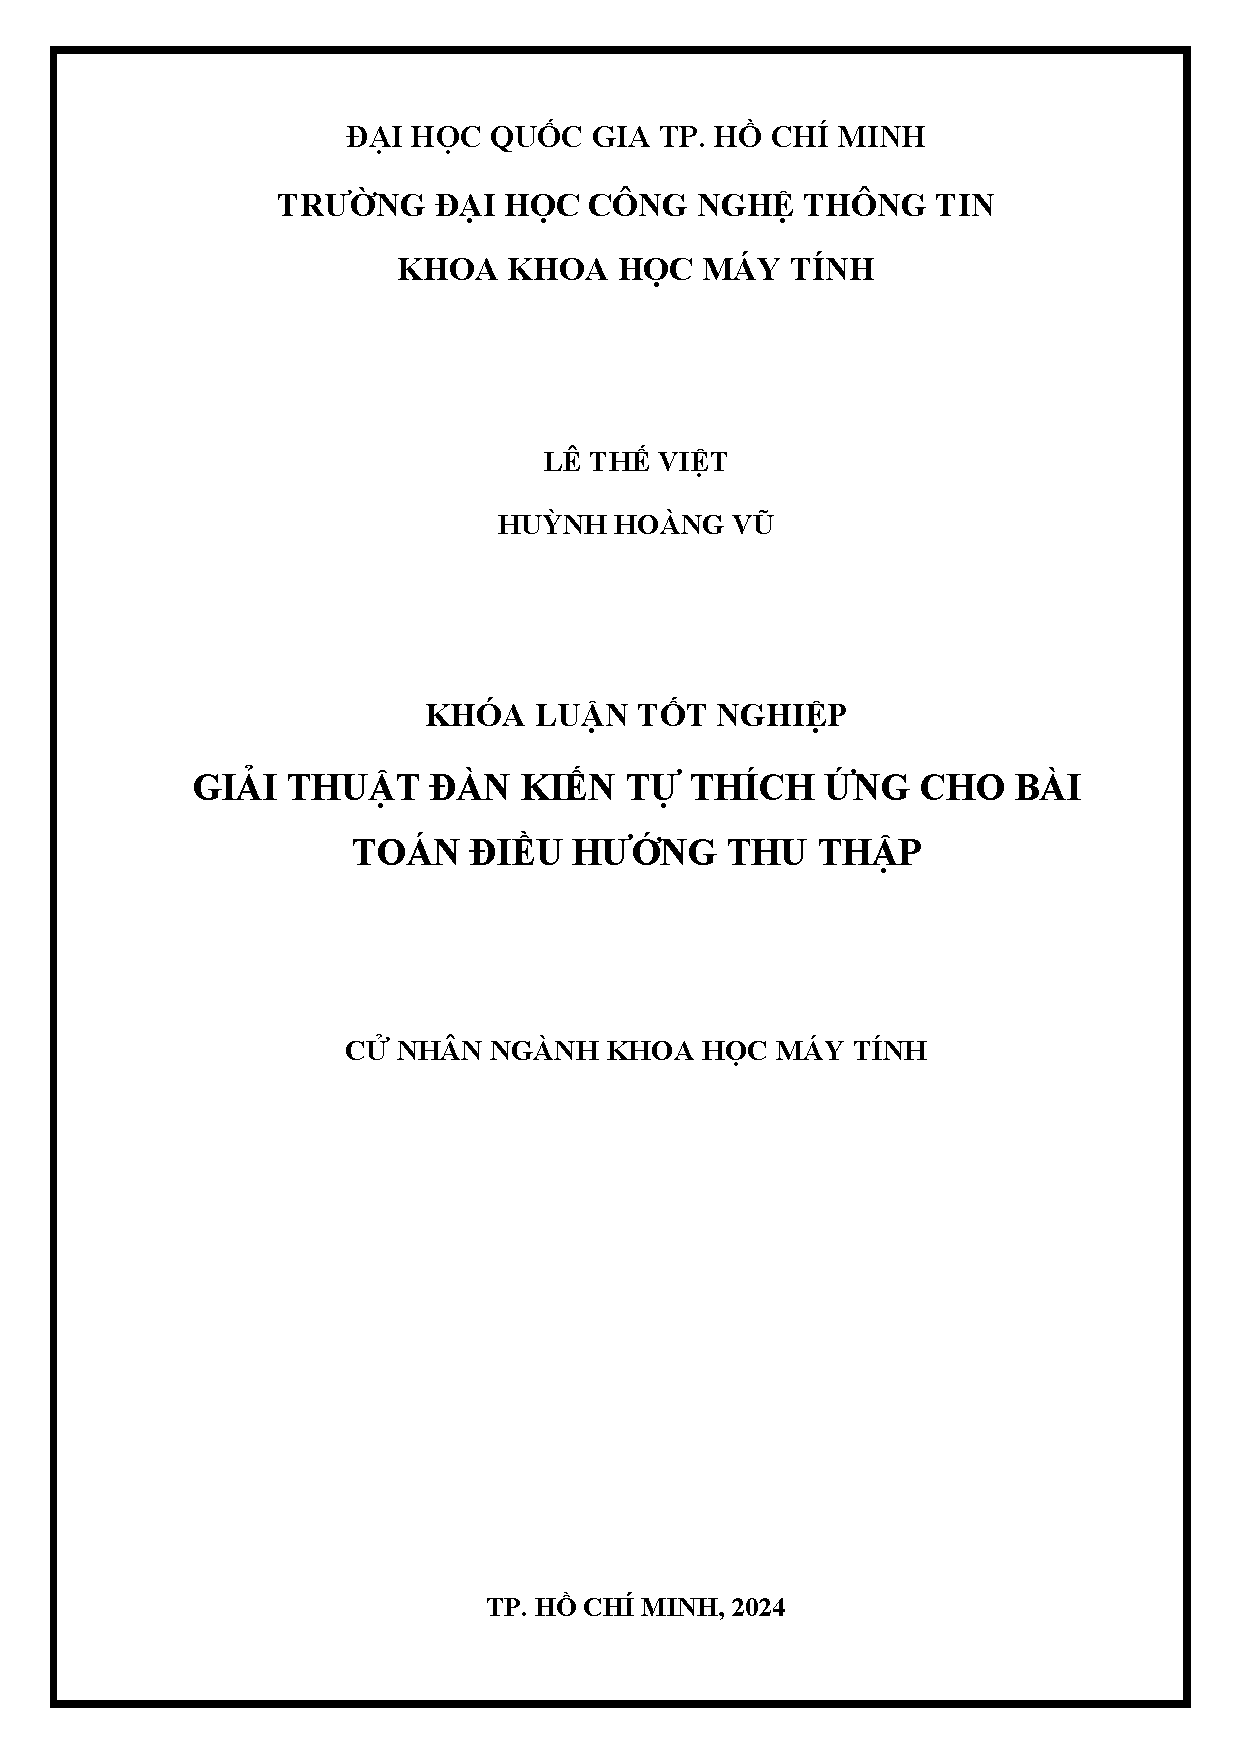
\includepdf[pages=-, scale=1]{TrangBia.pdf}
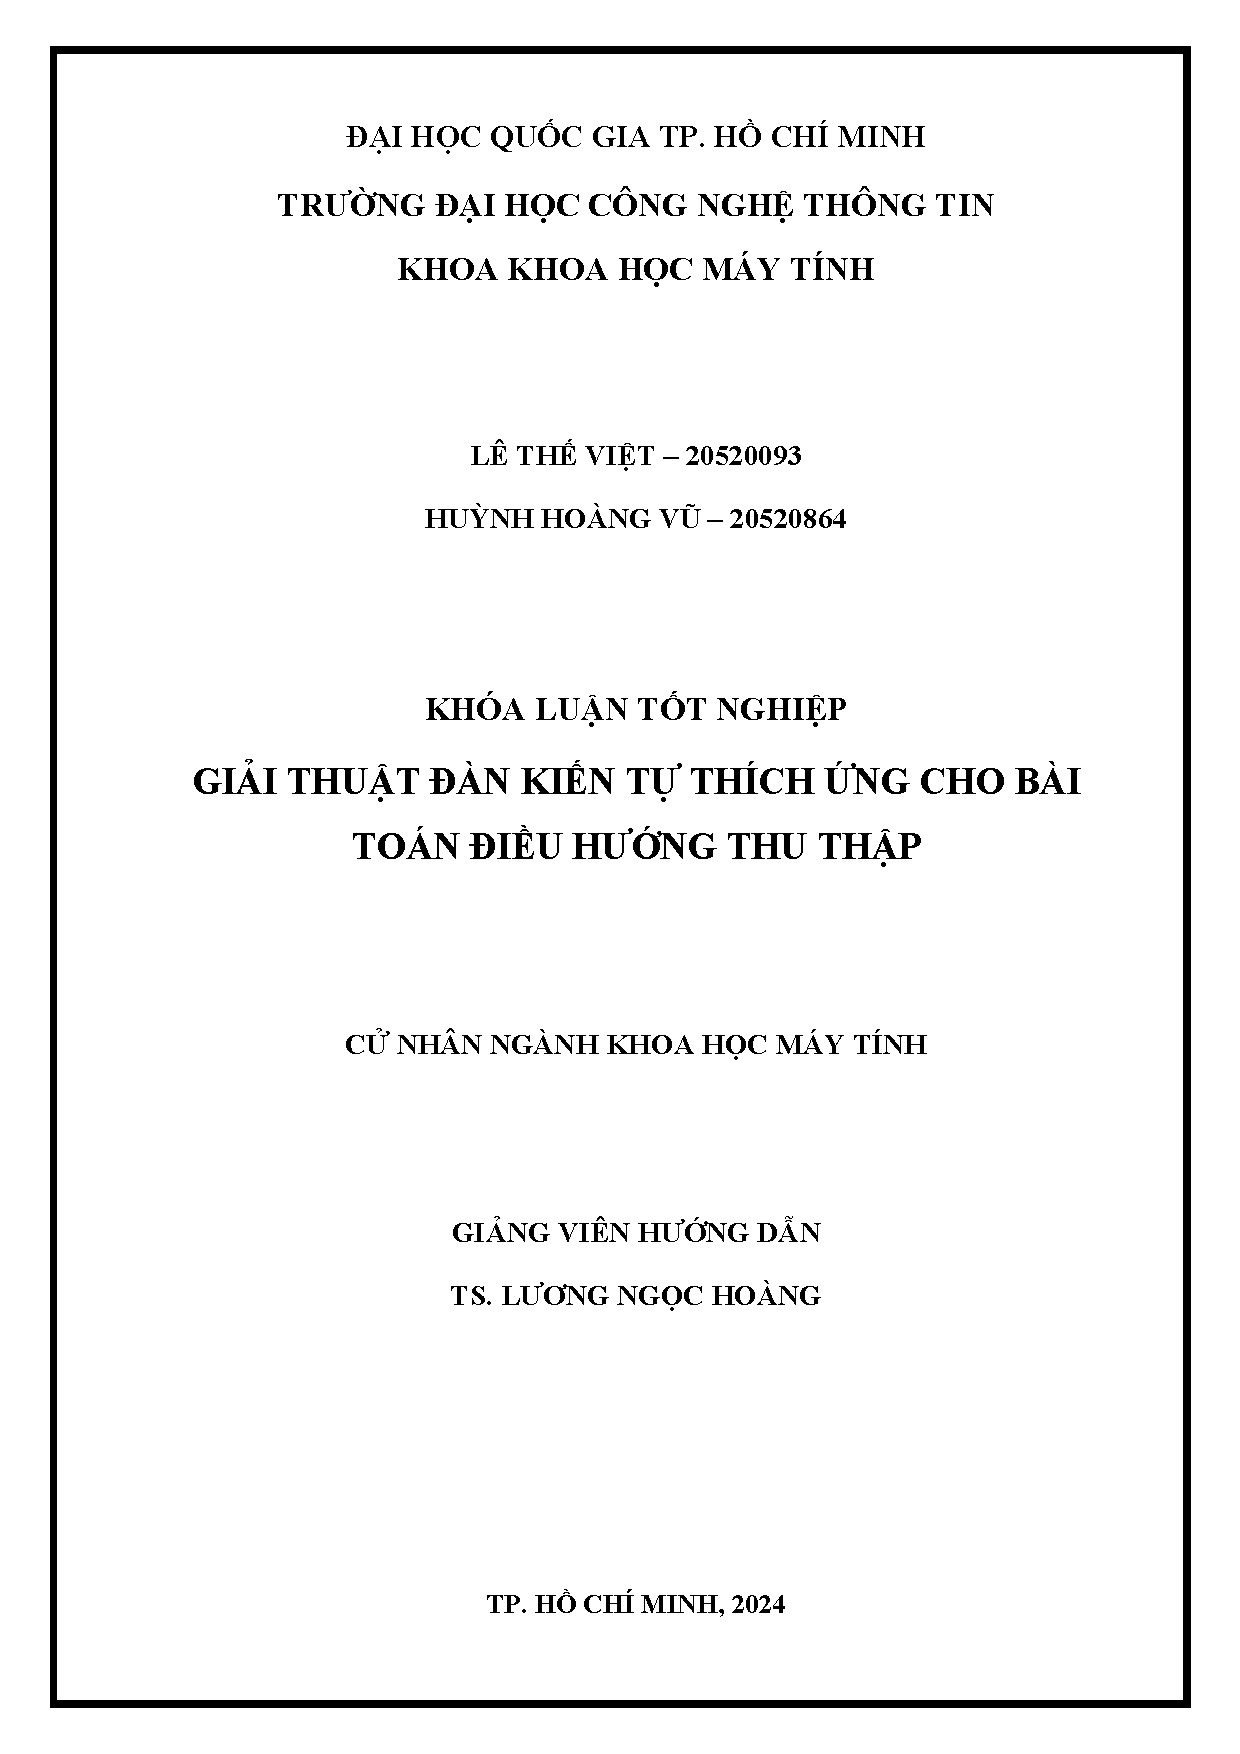
\includepdf[pages=-, scale=1]{TrangBia2.pdf}
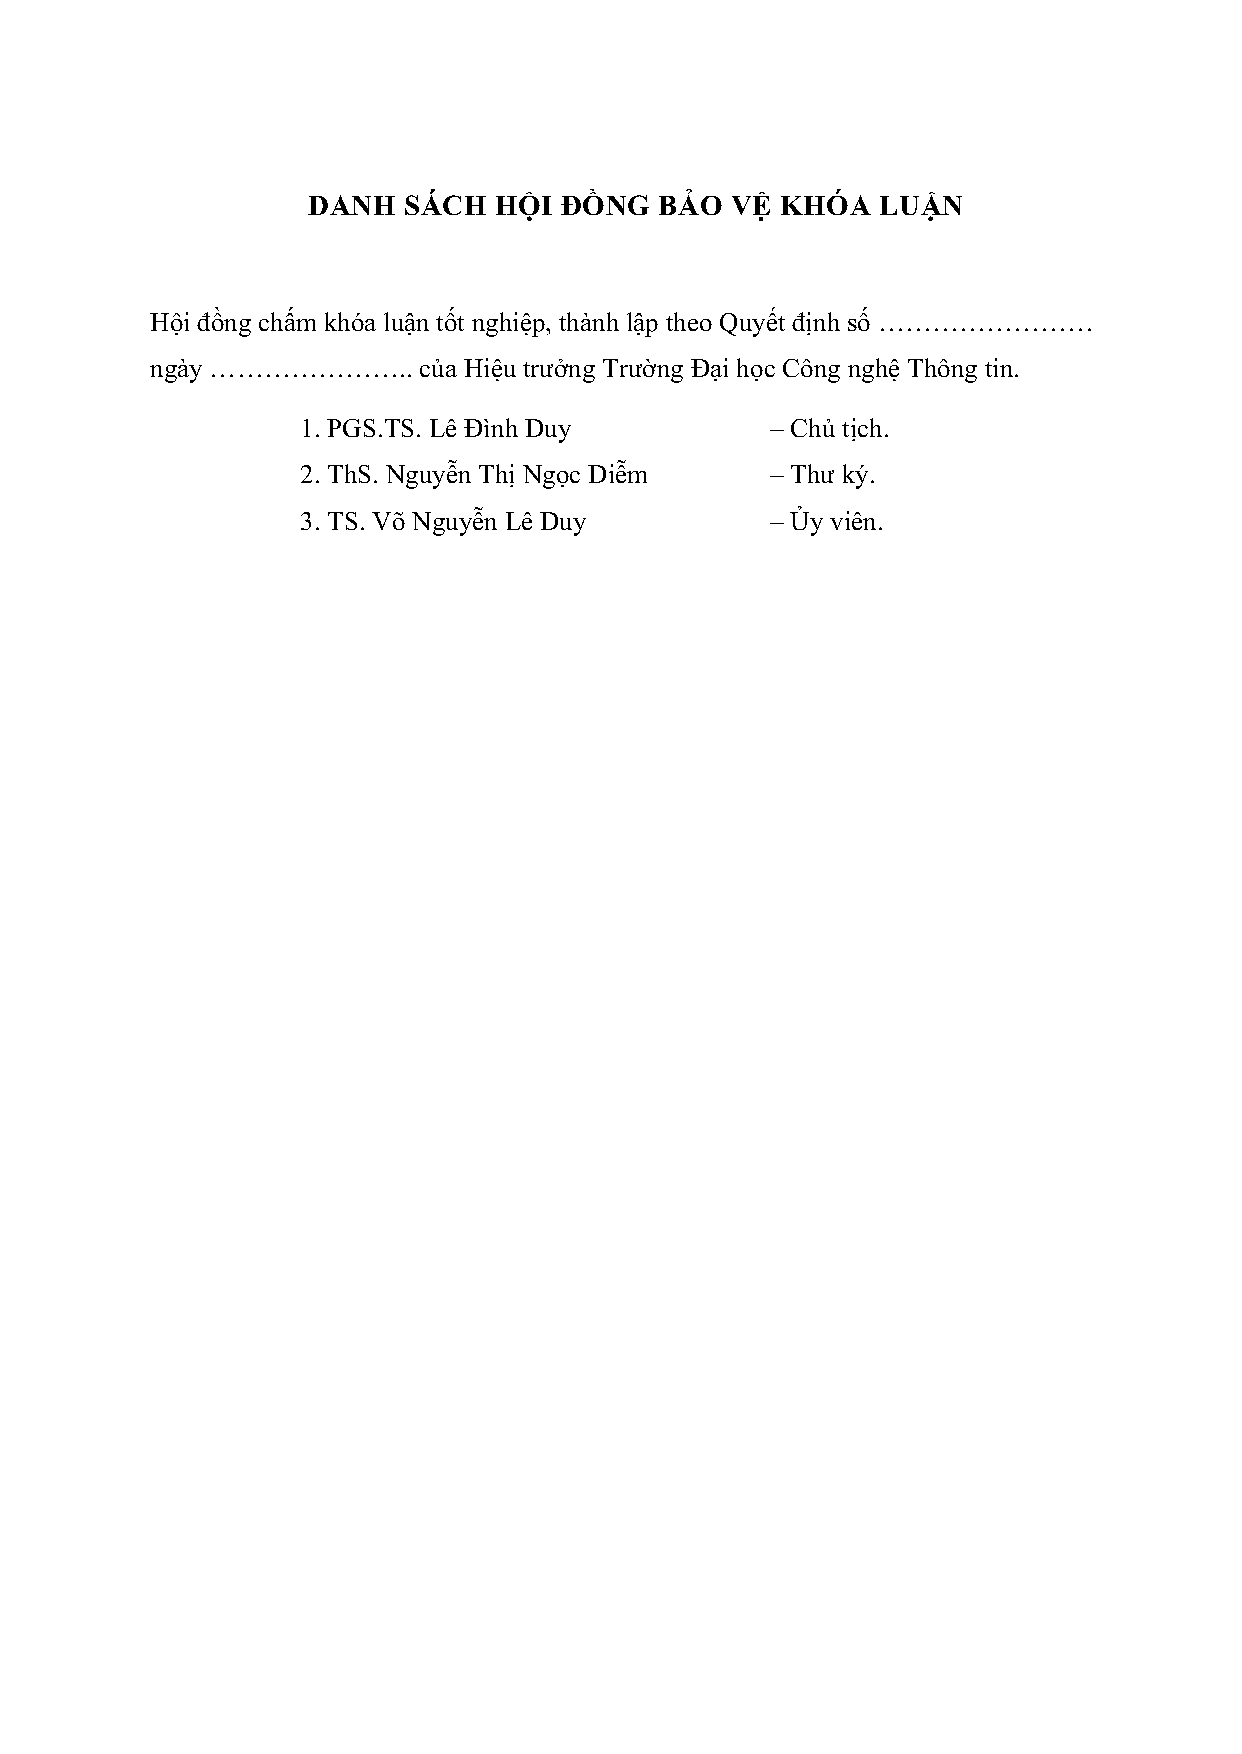
\includepdf[pages=-, scale=1]{DSHoiDong.pdf}
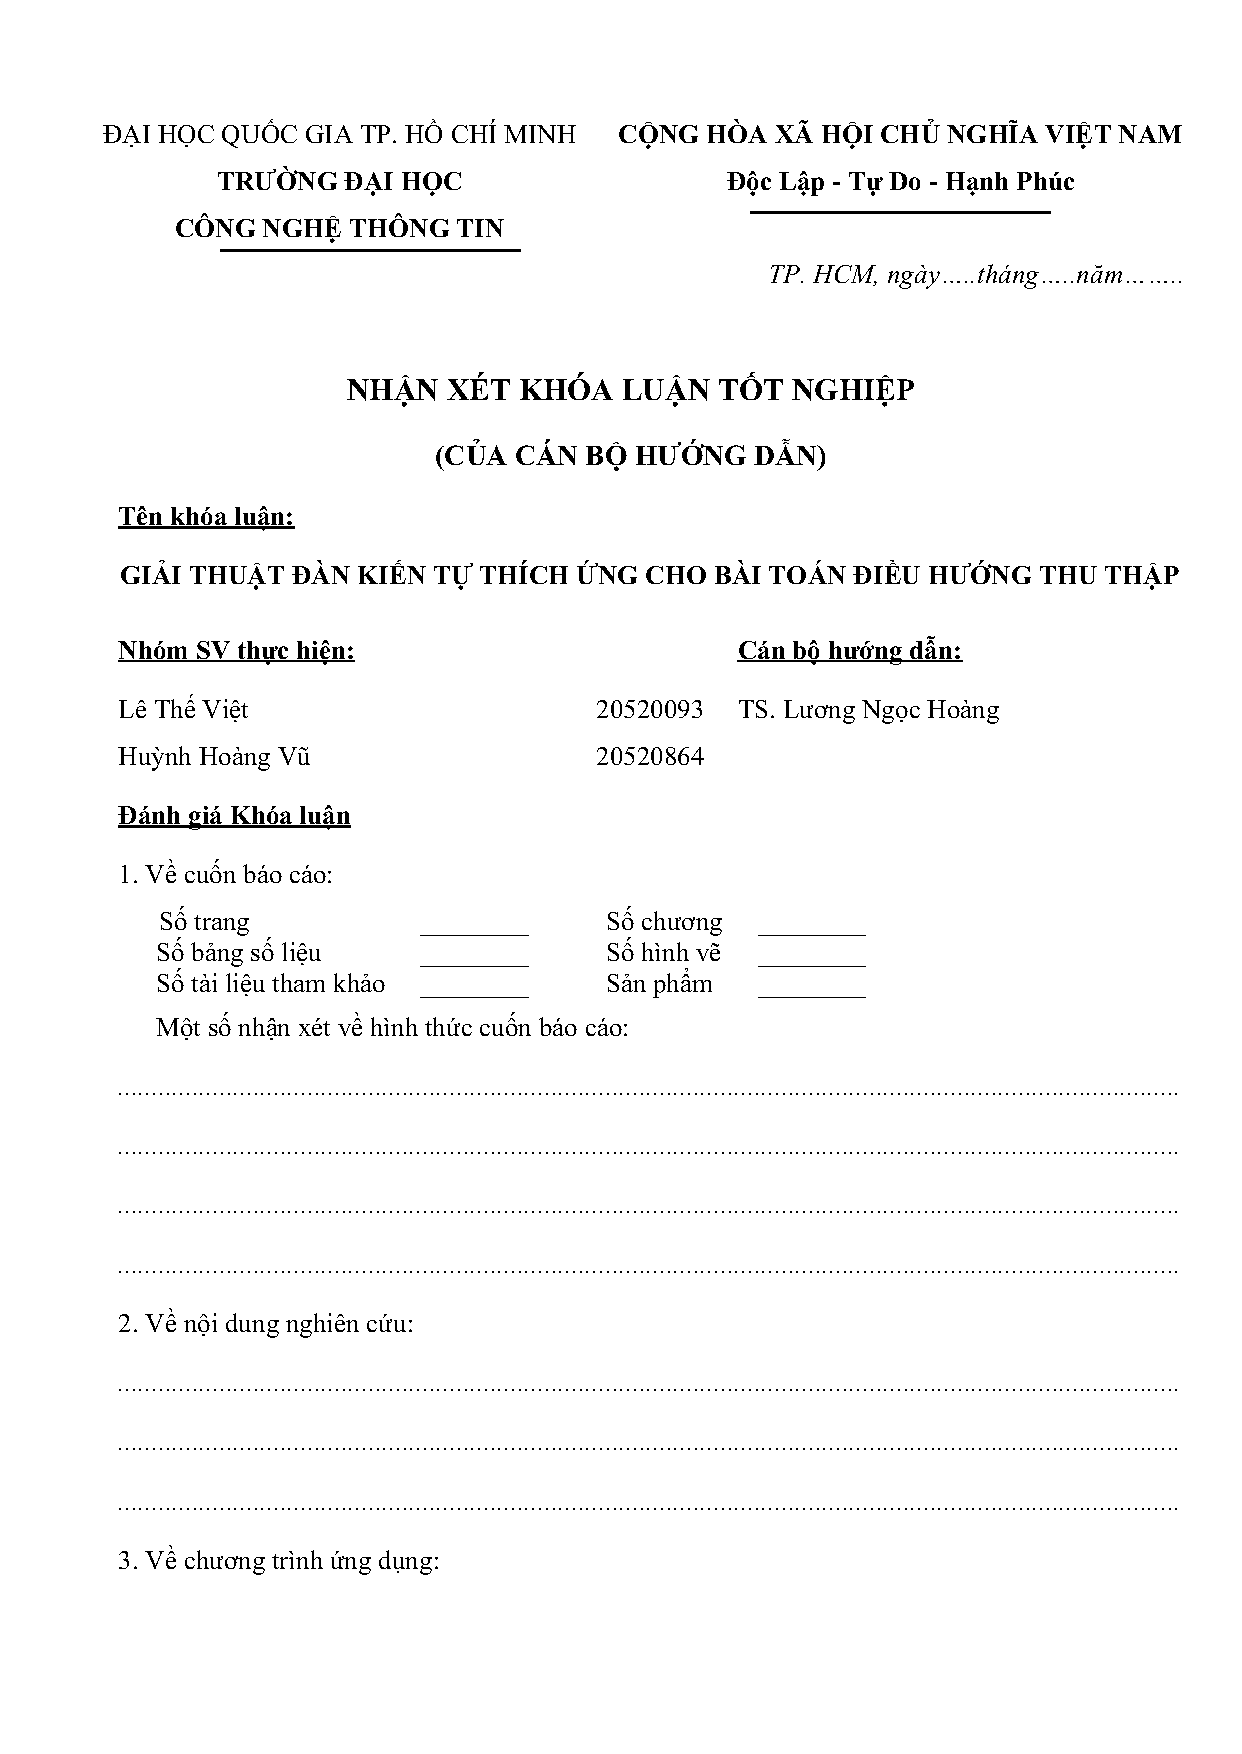
\includepdf[pages=-, scale=1]{NhanXetVaDeCuong.pdf}
\cleardoublepage
%--------------------------------

%	ACKNOWLEDGEMENTS
\begin{acknowledgements}
\addchaptertocentry{\ackname}
Chúng tôi chân thành bày tỏ lòng biết ơn đối với thầy Hoàng, TS. Lương Ngọc Hoàng, với sự kiên nhẫn và tận tâm hỗ trợ. Dưới sự hướng dẫn của thầy, chúng tôi đã đạt được kết quả nghiên cứu ấn tượng. Mặc dù nhiều lúc tiến độ thực hiện đề tài của chúng tôi gặp phải nhiều chậm trễ, nhưng thầy vẫn luôn tận tình hướng dẫn. Chân thành cảm ơn thầy.

Ngoài ra, chúng tôi cũng muốn bày tỏ lòng biết ơn đối với các thành viên trong nhóm nghiên cứu ELO và các bạn thuộc lớp KHTN2020. Các bạn là nguồn hỗ trợ tinh thần đáng quý khi được đồng hành cùng các bạn trong suốt quá trình học đại học cũng như quá trình thực hiện đề tài.

Cuối cùng, chúng tôi xin bày tỏ lòng biết ơn đến các thầy cô giảng viên và cán bộ công chức tại trường Đại học Công Nghệ Thông Tin. Sự nỗ lực hàng ngày của thầy cô đã tạo nên một môi trường học tập rèn luyện vô cùng bổ ích.

\end{acknowledgements}
%--------------------------------

%	LIST OF CONTENTS/FIGURES/TABLES PAGES
\renewcommand{\contentsname}{MỤC LỤC}
\tableofcontents % Prints the main table of contents
\cleardoublepage
% \addcontentsline{toc}{chapter}{\listfigurename}
\renewcommand{\listfigurename}{DANH SÁCH HÌNH VẼ}
\listoffigures % Prints the list of figures
\cleardoublepage
% \addcontentsline{toc}{chapter}{\listtablename}
\renewcommand{\listtablename}{DANH SÁCH BẢNG}
\listoftables % Prints the list of tables
\cleardoublepage
%--------------------------------

%	ABBREVIATIONS
% \addchaptertocentry{\abbrevname}
\begin{abbreviations}{ll} % Include a list of abbreviations (a table of two columns)
\textbf{AACO-NC} & \textbf{A}daptive \textbf{A}nt \textbf{C}olony \textbf{O}ptimization with \textbf{n}ode \textbf{c}lustering \\
\textbf{ACO++} & MAX-MIN ant colony optimization for ThOP \\
\textbf{ACO} & \textbf{A}nt \textbf{C}olony \textbf{O}ptimization\\
\textbf{BRKGA} & \textbf{B}iased \textbf{R}andom-\textbf{K}ey \textbf{G}enetic \textbf{A}lgorithm \\
\textbf{CMA-ES} & \textbf{C}ovariance \textbf{M}atrix \textbf{A}daptation \textbf{E}volution \textbf{S}trategy \\
\textbf{ES} & \textbf{E}volution \textbf{S}trategy \\
\textbf{GA} & \textbf{G}enetic \textbf{A}lgorithm \\
\textbf{ILS} & \textbf{I}terated \textbf{L}ocal \textbf{S}earch \\
\textbf{KP} & \textbf{K}napsack \textbf{P}roblem \\
\textbf{MINLP} & \textbf{M}ixed \textbf{I}nteger {N}on-\textbf{L}inear \textbf{P}rogramming \\
\textbf{MMAS} & \textbf{M}AX-\textbf{M}IN \textbf{a}nt \textbf{s}ystem\\
\textbf{OP} & \textbf{O}rienteering \textbf{P}roblem\\
\textbf{SAAS} & \textbf{S}elf-\textbf{A}daptive \textbf{A}nt \textbf{S}ystem\\
\textbf{TSP} & \textbf{T}raveling {S}alesman {P}roblem \\
\textbf{TTP} & \textbf{Th}ief \textbf{T}raveling \textbf{P}roblem\\
\textbf{ThOP} & \textbf{Th}ief \textbf{O}rienteering \textbf{P}roblem\\

\end{abbreviations}
%--------------------------------

%	ABSTRACT
\begin{abstract}
\addchaptertocentry{\titleAbstract}

Bài toán Điều Hướng Thu Thập (Thief Orienteering Problem) là một vấn đề đa thành phần với hai bài toán con tương tác là bài toán Ba Lô (Knapsack Problem) và bài toán Điều Hướng (Orienteering Problem). ACO++, một metaheuristic hiện đại cho ThOP, kết hợp thuật toán MAX-MIN Ant System để xây dựng đường đi, một thuật toán ngẫu nhiên cho việc tạo chiến lược thu thập, và phương pháp 2-OPT cho tìm kiếm cục bộ (local search). Tuy nhiên, hiệu suất xuất sắc được báo cáo của ACO++ được đạt được bằng cách sử dụng các bộ giá trị tham số khác nhau đã được điều chỉnh tỉ mỉ cho từng nhóm cụ thể của các trường hợp đánh giá. Trong công trình này, chúng tôi đề xuất một biến thể tự thích ứng mới của ACO++. Không đòi hỏi quá trình điều chỉnh phức tạp, phương pháp của chúng tôi sử dụng các cơ chế thích ứng để điều chỉnh các tham số cho từng trường hợp vấn đề cụ thể trong quá trình chạy thuật toán. Chúng tôi cũng sử dụng kỹ thuật bay hơi lười biếng và tận dụng phân cụm thứ bậc để cải thiện hiệu suất của đàn kiến trong việc khám phá không gian tìm kiếm. Trong số 432 trường hợp đánh giá, phương pháp Self-Adaptive Ant System (SAAS) của chúng tôi tạo ra kết quả vượt trội hơn so với các phương pháp tân tiến trước đó. Mã nguồn đã được công bố tại \url{https://github.com/ELO-Lab/SAAS-HC}.

\end{abstract}
%--------------------------------

%	THESIS CONTENT - CHAPTERS
\mainmatter % Begin numeric (1,2,3...) page numbering

\pagestyle{thesis} % Return the page headers back to the "thesis" style
\def\vec#1{\mathchoice{\mbox{\boldmath$\displaystyle#1$}}
{\mbox{\boldmath$\textstyle#1$}}
{\mbox{\boldmath$\scriptstyle#1$}}
{\mbox{\boldmath$\scriptscriptstyle#1$}}}
\renewcommand{\chaptername}{Chương}
\renewcommand{\figurename}{Hình}
\renewcommand{\tablename}{Bảng}
\renewcommand{\bibname}{TÀI LIỆU THAM KHẢO}
\makeatletter
% \renewcommand*{\ALG@name}{Thuật giải}
\renewcommand{\algorithmcfname}{Giải thuật}
\makeatother
\chapter{TỔNG QUAN} \label{chapter:Introduction}

\section{Đối tượng nghiên cứu}

Các bài toán đa thành phần liên quan đến nhiều thành phần tương tác và phổ biến trong các tình huống thực tế, như định tuyến xe có ràng buộc về tải trọng \cite{doi:10.1287/trsc.1060.0165} hoặc tối ưu hóa việc sử dụng vật liệu trong lịch trình sản xuất \cite{10.1007/978-3-642-21827-9_23}. Những vấn đề này tạo thách thức do sự phụ thuộc lẫn nhau giữa các thành phần và thường liên quan đến các nhiệm vụ tối ưu hóa NP-Hard như đóng gói, lập lịch và định tuyến \cite{Bonyadi2019}. Bài toán Người Thu Thập Du Lịch (Thief Traveling Problem, TTP) \cite{6557681} là một vấn đề đa thành phần đặc trưng kết hợp bài toán Ba Lô (Knapsack Problem, KP) và bài toán Người Bán Hàng Du Lịch (Traveling Salesman Problem, TSP).

Trong công trình này, chúng tôi giải quyết bài toán Điều Hướng Thu Thập (Thief Orienteering Problem, ThOP) \cite{8477853}, một vấn đề đa thành phần được biến thể từ TTP với các tương tác và ràng buộc mới. ThOP kết hợp bài toán Điều hướng (Orienteering Problem, OP) \cite{OP} và KP. Mục tiêu là tìm một tuyến đường từ thành phố xuất phát đến thành phố đích (thành phần OP) sao cho tối đa hóa tổng lợi nhuận của các vật phẩm được thu thập (thành phần KP), đồng thời tuân thủ giới hạn sức chứa của ba lô và giới hạn thời gian di chuyển. ThOP được lấy cảm hứng từ TTP và xem xét các tình huống thực tế nơi người thu thập không cần phải ghé thăm tất cả các thành phố và tương tác được xác định bởi thời gian và giới hạn của ba lô. Vấn đề này được ứng dụng trong logistics ngược (reverse logistics) \cite{8477853}, nơi công ty cần thu nhận hàng hóa từ khách hàng, mỗi món hàng mang lại lợi ích cụ thể, dưới sự giới hạn của khả năng chở hàng và giờ làm việc của tài xế.

\section{Phạm vi nghiên cứu}

Chúng tôi tập trung nghiên cứu các giải pháp với hướng tiếp cận heuristic, metaheuristic cho ThOP. Các thuật toán heuristic giúp ta đạt được kết quả tương đối tốt với chi phí thời gian chấp nhận được. Chúng trái ngược với các phương pháp chính xác (exact methods), cái mà sẽ đảm bảo tìm được lời giải tối ưu. Đối với bài toán NP-Hard như ThOP, thời gian chạy cần thiết của phương pháp chính xác sẽ tăng nhanh chóng với kích thước của bài toán dẫn đến không khả thi để ứng dụng vào thực tế. Do đó, nghiên cứu giải pháp heuristic sẽ có tính ứng dụng cao hơn.

Bên cạnh hướng tiếp cận thuật toán, chúng tôi đã tiến hành thực nghiệm trên Bộ trường hợp đánh giá do Santos và Chagas thiết kế \cite{8477853} khi giới thiệu ThOP. Nó bao gồm 432 thể hiện của bài toán Điều Hướng Thu Thập với đa dạng về số lượng thành phố, số lượng vật phẩm, kích thước ba lô, thời gian di chuyển tối đa và sự tương quan giữa trọng lượng và lợi nhuận của các vật phẩm. 

\section{Các công trình liên quan}

Các công trước đây cho ThOP đa dạng về hướng tiếp cận. Một phương pháp chính xác Lập Trình Phi Tuyến Tính Hỗn Hợp (Mixed Integer Non-Linear Programming, MINLP) \cite{8477853}. Một phương pháp tìm kiếm cục bộ Tìm Kiếm Cục Bộ Tuần Tự (Iterated Local Search, ILS) \cite{8477853}. Hai phương pháp thuật giải di truyền Thuật Giải Di Truyền Điểm Thiên Lệch Ngẫu Nhiên (Biased Random-Key Genetic Algorithm, BRKGA) \cite{8477853}, Thuật Giải Di Truyền (Genetic Algorithm, GA) \cite{9185848}. Một phương pháp thông minh bầy đàn Giải Thuật Tối Ưu Hóa Đàn Kiến (Ant Colony Optimization, ACO) \cite{CHAGAS2020708}. Và sự kết hợp giữa thông minh bầy đàn và tìm kiếm cục bộ ACO++ \cite{Chagas2021}. 

Chagas và Wagner \cite{Chagas2021} đã chỉ ra rằng ACO++ vượt trội hơn so với các thuật toán khác trong hơn 90\% số lượng trường hợp (trường hợp đánh giá). Để đạt được những kết quả xuất sắc này, ACO++ trải qua quá trình điều chỉnh chi tiết để xác định cấu hình siêu tham số phù hợp cho mỗi nhóm trường hợp trong benchmark (bộ đánh giá) của ThOP.

\section{Mục đích nghiên cứu}

Trong công trình này, chúng tôi đề xuất một thuật toán cải tiến dựa trên ACO++, Giải Thuật Đàn Kiến Tự Thích Ứng (Self-Adaptive Ant System, SAAS) có khả năng điều chỉnh động các tham số của mình theo đặc trưng của mỗi trường hợp và quá trình tìm kiếm. Sự cải tiến này giúp giảm thiểu tính tốn thời gian và phi thực tế của việc điều chỉnh nhiều cấu hình siêu tham số. Thuật toán của chúng tôi sử dụng một cấu hình duy nhất cho toàn bộ trường hợp trong ThOP benchmark, đồng thời mang lại hiệu suất vượt trội.

Đề cải tiến, chúng tôi tích hợp bốn kỹ thuật vào ACO++. Hai cơ chế kiểm soát tham số, tự thích ứng (self-adaptive) và thích ứng (adaptive), giúp cải thiện khả năng thích nghi của thuật toán. Hai kỹ thuật Bay hơi lười biếng và Phân cụm thứ bậc giúp giảm độ phức tạp về thời gian.

Cơ chế tự thích ứng sử dụng chiến lược tiến hóa (Evolution Strategy, ES), trong khi đó cơ chế thích ứng sử dụng thông tin sự đa dạng lợi nhuận để điều chỉnh các tham số (Bảng \ref{tab:control_param}). Các tham số được điều chỉnh đồng thời với quá trình tìm kiếm lời giải. Phân cụm phân cấp được sử dụng để giảm chi phí xây dựng các tuyến đường. Bay hơi lười biếng được sử dụng để giảm thời gian cần thiết để bay hơi dấu vết pheromone của kiến.

\chapter{KIẾN THỨC NỀN TẢNG} \label{chapter:BasedKnowledge}
Ở chương này, chúng tôi sẽ cung cấp các kiến thức được sử dụng xuyên suốt trong khóa luận này. Ở phần \ref{section:ProblemDefinition}, chúng tôi sẽ mô tả chi tiết bài toán mà chúng tôi giải quyết, bài toán Điều Hướng Thu Thập. Chúng tôi sẽ trình bày thế nào là một bài toán tối ưu hóa đa thành phần, các bài toán con, các mục tiêu đặt ra khi giải quyết bài toán này. Ở phần \ref{section:ACO}, chúng tôi sẽ trình bày các kiến thức nền tảng về giải thuật tối ưu hóa đàn kiến và biến thể MAX-MIN ACO của nó, thuật toán mà chúng tôi sử dụng làm nền tảng để phát triển nên thuật toán chúng tôi đề xuất. Bên cạnh đó chúng tôi trình bày các kiến thức cơ sở của các phương pháp chúng tôi sử dụng để thích ứng các tham số (phần \ref{section:AdaptivePheromoneRate}, \ref{section:bgCMA-ES} và \ref{section:parametersetting}) và làm giảm độ phức tạp của thuật toán (phần \ref{section:bgClusterTree}).
\section{Bài toán Điều Hướng Thu Thập}\label{section:ProblemDefinition}
\subsection{Mô tả bài toán}
Bài toán chúng tôi giải quyết ở công trình này là bài toán Điều Hướng Thu Thập (Thief Orienteering Problem, ThOP), là một biến thể của bài toán Điều Hướng (Orienteering Problem) được lấy cảm hứng từ bài toán Người Thu Thập Du Lịch (Travelling Thief Problem, TTP). TTP được đề xuất  bởi Bonyadi, Michalewicz và Barone \cite{6557681}. Đây là sự kết hợp của hai bài toán kinh điển nổi tiếng: bài toán Người Bán Hàng Du lịch (Traveling Salesman Problem, TSP) và bài toán Ba Lô (Knapsack Problem, KP). Điểm chính mà tác giả trình bày để đề xuất TTP là các thang đo của các bài toán NP-Hard kinh điển không phản ánh đúng các đặc điểm chính của các vấn đề thực tế, nên các thuật toán metaheuristics hiệu quả mà chúng ta có cho những thang đo đó không nhất thiết hiệu quả cho các vấn đề thực tế. Tác giả cho rằng sự phức tạp của các vấn đề thực tế không chỉ đến từ kích thước của chúng, mà chủ yếu là do chúng là sự kết hợp của hai hoặc nhiều vấn đề tối ưu hóa con, và vì những vấn đề con đó là tương phụ thuộc lẫn nhau. Điều này có nghĩa là việc giải quyết một vấn đề con ảnh hưởng đến chất lượng của việc giải quyết các vấn đề con khác, do đó chúng không nên được giải quyết độc lập. Trong TTP, một người thu thập phải ghé thăm mỗi thành phố trong một tập hợp gồm n thành phố (bài toán con TSP) và trong quá trình ghé thăm có thể thu thập các vật phẩm nằm ở các thành phố đó để đựng trong ba lô của mình (bài toán con KP). Tuy nhiên, khi các vật phẩm được thu thập, balo trở nên nặng hơn và người thu thập đi chậm hơn. Ba lô của người thu thập thuê, và giá phải trả là tỉ lệ với thời gian thuê. Người thu thập sau đó phải tối đa hóa tổng lợi nhuận của các vật phẩm đã thu thập và đồng thời giảm thiểu tổng thời gian của hành trình. Tác giả chỉ ra rằng giải pháp tối ưu của một trường hợp TTP có thể không bao gồm giải pháp tối ưu của bài toán con KP hoặc bài toán con TSP, chứng minh sự phụ thuộc lẫn nhau của các bài toán con trong đó.

Lấy cảm hứng từ TTP, Santos và Changas \cite{8477853} giới thiệu ở một bài toán đa thành phần mới, đó là bài toán Điều Hướng Thu Thập (ThOP), được xây dựng trên cơ sở của bài toán Điều Hướng (OP) thay vì bài toán Người Bán Hàng Du Lịch như TTP. Bài toán Điều Hướng dựa trên một trò chơi thể thao địa hình. Trong trò chơi, các đối thủ bắt đầu từ một điểm cho trước, đi qua một khu vực ghé thăm các điểm kiểm tra và phải quay lại một điểm kiểm soát trong một khoảng thời gian nhất định. Họ có một bản đồ của khu vực và phải tự quyết định tuyến đường qua các điểm kiểm tra dựa trên kỹ năng định hình và cấp độ thể dục của họ. Trong OP, mỗi điểm kiểm tra có điểm số, vì vậy mục tiêu là tìm ra tuyến đường tối đa hóa tổng điểm số, tức là tổng số điểm của các điểm kiểm tra đã ghé thăm là tối đa. Trong biến thể ThOP, một đối thủ hay chúng tôi gọi là người thu thập không ghi điểm chỉ bằng cách ghé thăm các điểm trên bản đồ, mà phải thu thập các vật phẩm tại các điểm và mang theo chúng đến điểm kết thúc. Mỗi đối thủ có một ba lô với sức chứa giới hạn cho các vật phẩm được thu thập. Hơn nữa, tốc độ của người thu thập bị ảnh hưởng trực tiếp bởi trọng lượng của ba lô. Như ở bài toán TTP, khi các vật phẩm được thu thập, ba lô sẽ nặng dần, và tốc độ của người thu thập sẽ giảm xuống. Gọi $v_{min}$, $v_{max}$ là tốc độ tối thiểu và tốc độ tối đa mà người thu thập di chuyển tương ứng khi ba lô đạt sức chứa giới hạn $W$ hoặc ba lô rỗng. Tốc độ di chuyển $v$ của người thu thập với ba lô có sức nặng $w$, $0 \leq w \leq W$ được tính bằng $v = v_{max} - w \cdot(v_{max} - v_{min})/W$. Lưu ý rằng giá trị $(v_{max} - v_{min})/W$ là hằng số và thể hiện độ giảm của tốc độ với một đơn vị cân nặng của ba lô.

Mục tiêu của ThOP là cung cấp một đường đi từ thành phố bắt đầu 1 đến thành phố kết thúc n, cũng như một tập các vật phẩm được chọn từ các thành phố đã ghé thăm trong suốt hành trình để tối đa hóa tổng lợi nhuận đã lấy, đồng thời đảm bảo rằng sức chứa của balo không vượt quá sức chứa giới hạn $W$ và tổng thời gian di chuyển của người thu thập nằm trong giới hạn thời gian $T$. Người thu thập không cần phải ghé thăm tất cả các thành phố.

\begin{figure}[ht!]
    \centering
    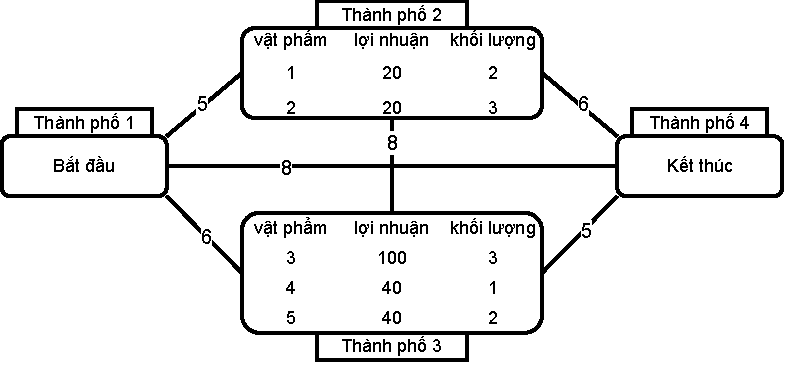
\includegraphics[width=\textwidth]{Figures/ThOP-instance.pdf}
    \caption[Minh họa một ví dụ của bài toán Điều Hướng Thu Thập.]{Minh họa một ví dụ của bài toán Điều Hướng Thu Thập bao gồm 4 thành phố, 5 vật phẩm.}
    \label{fig:ThOPinstance}
\end{figure}

Để hiểu rõ bài toán Điều Hướng Thu Thập ThOP, chúng tôi minh họa trong hình \ref{fig:ThOPinstance} một ví dụ nhỏ của một trường hợp ThOP liên quan đến 4 thành phố và 5 vật phẩm. Lưu ý rằng không có vật phẩm nào ở thành phố bắt đầu (1) và thành phố kết thúc (4), các số vật phẩm có trọng lượng và lợi nhuận khác nhau được phân phối ở các thành phố khác (2 và 3). Các khoảng cách từ mỗi cặp thành phố được cho trong các cạnh. Dưới đây, chúng tôi trình bày chi tiết một số lời giải cho trường hợp này. Chúng tôi đặt các ràng buộc của ví dụ này như sau: $v_{min} = 0.1$, $v_{max} = 1.0$, $W = 3$ và $T = 75$.

Chúng tôi biểu diễn một lời giải cho bài toán ThOP dưới dạng hai phần ($\pi$, $z$). Phần đầu tiên bao gồm tuyến đường di chuyển của người thu thập $\pi = \langle 1, \pi_2, \pi_3, ..., \\\pi_k, n \rangle$, một véc tơ chứa danh sách thành phố đã ghé thăm theo thứ tự di chuyển. Lưu ý rằng thành phố đầu tiên và cuối cùng được cố định cho mọi lời giải hợp lệ. Phần thứ hai là chiến lược thu thập vật phẩm $z = \langle z_1, z_2, . . . , z_m \rangle$, một véc tơ nhị phân đại diện cho trạng thái của các vật phẩm ($z_i = 1$ nếu vật phẩm i được lấy, và 0 nếu ngược lại). Theo biểu diễn này, hãy xem xét các lời giải ThOP sau cho trường hợp đã mô tả ở trên:
\begin{itemize}
    \item $(\langle1,2,3,4\rangle,\langle1,0,0,1,0\rangle)$: là một lời giải hợp lệ với tổng lợi nhuận là $20+40=60$. Tổng khối lượng các vật phẩm được thu thập là 3 và thời gian di chuyển là 75, thỏa mãn cả hai ràng buộc giới hạn sức chứa ba lô $W$ và thời gian di chuyển $T$. Tổng thời gian di chuyển được tính như sau:
    \begin{itemize}
        \item di chuyển từ thành phố bắt đầu đến thành phố thứ 2 với tốc độ tối đa: thời gian di chuyển là $d_{12}/v_{max}=5/1.0=5$ 
    	\item tại thành phố thứ 2, người thu thập lấy vật phẩm 1: vận tốc giảm xuống $v=1.0-2\times(1.0-0.1)/3=0.4$ 
    	\item di chuyển từ thành phố thứ 2 sang thành phố thứ 3: tổng thời gian di chuyển là $5+d_{23}/v=5+8/0.4=5+20=25$ 
    	\item tại thành phố thứ 3, vật phẩm thứ 4 được lấy: vận tốc giảm xuống $v=1.0-3\times(1.0-0.1)/3=0.1$ 
    	\item di chuyển từ thành phố thứ 3 đến thành phố kết thúc 4: tổng thời gian di chuyển là $5+20+d_{34}/v=5+20+5/0.1=5+20+50=75$ 
    \end{itemize}
    \item $(\langle1,3,2,4\rangle,\langle1,0,0,1,0\rangle)$: là một lời giải không hợp lệ. Mặc dù chiến lược thu thập với lời giải ơ trên nhưng tổng thời gian di chuyển (83.43) vượt quá ràng buộc thời gian:
    \begin{itemize}
        \item di chuyển từ thành phố bắt đầu đến thành phố thứ 3 với tốc độ tối đa: thời gian di chuyển là $d_{13}/v_{max}=6/1.0=6$ 
    	\item tại thành phố thứ 3, người thu thập lấy vật phẩm 4: vận tốc giảm xuống $v=1.0-1\times(1.0-0.1)/3=0.7$ 
    	\item di chuyển từ thành phố thứ 3 sang thành phố thứ 2: tổng thời gian di chuyển là $6+d_{32}/v=6+8/0.7=6+11.43=17.43$ 
    	\item tại thành phố thứ 2, vật phẩm thứ 1 được lấy: vận tốc giảm xuống $v=1.0-3\times(1.0-0.1)/3=0.1$ 
    	\item di chuyển từ thành phố thứ 2 đến thành phố kết thúc 4: tổng thời gian di chuyển là $6+17.43+d_{24}/v=6+17.43+6/0.1=83.43$ 
    \end{itemize}
	\item $(\langle1,3,4\rangle,\langle0,0,1,0,0\rangle)$: là một lời giải tối ưu cho trường hợp ví dụ này với tổng lợi nhuận là 100. Tổng khối lượng ba lô là $3\leq W$ và tổng thời gian di chuyển là $56 \leq T$:
    \begin{itemize}
        \item di chuyển từ thành phố bắt đầu đến thành phố thứ 3 với tốc độ tối đa: thời gian di chuyển là $d_{13}/v_{max}=6/1.0=6$ 
        \item tại thành phố thứ 3, người thu thập lấy vật phẩm 3: vận tốc giảm xuống $v=1.0-3\times(1.0-0.1)/3=0.1$ 
        \item di chuyển từ thành phố thứ 3 đến thành phố kết thúc 4: tổng thời gian di chuyển là $6+d_{34}/v=6+5/0.1=6+50=56$ 
    \end{itemize}
\end{itemize}

Lưu ý rằng chiến lược thu thập của lời giải tối ưu cho trường hợp ví dụ giống như lời giải tối ưu cho bài toán con Ba Lô. Tuy nhiên, không phải lúc nào người thu thập cũng có chiến lược thu thập vật phẩm tốt nhất giống với lời giải tốt ưu cho bài toán con Ba Lô trong giới hạn thời gian $T$. Để minh họa điều này, hãy xem xét một giới hạn thời gian chặt chẽ hơn là 20 với ví dụ trước đó. Trong trường hợp này, lời giải  tối ưu sẽ là $(\langle1, 3, 4\rangle, \langle0, 0, 0, 1, 1\rangle)$, có tổng lợi nhuận là 80 và tổng thời gian di chuyển là 18.5.
\subsection{Biểu diễn toán học}
Ở phần này chúng tôi trình bày mô hình bài toán Điều Hướng Thu Thập dưới dạng công thức toán học không tuyến tính. Với bài toán ThOP, chúng ta có một tập hợp gồm $n$ thành phố: 1 là thành phố bắt đầu, $n$ là thành phố kết thúc, và các thành phố còn lại $(2, . . . , n - 1)$ là các thành phố trung gian. Tại mỗi thành phố trung gian có một hoặc nhiều vật phẩm, và đối với mỗi vật phẩm $i$, chúng ta có lợi nhuận $p_i$ và trọng lượng $w_i$ của nó. Chúng ta cũng được cho biết giới hạn sức chứa $W$ của ba lô, giới hạn thời gian di chuyển $T$ để đến thành phố kết thúc, tốc độ tối đa và tối thiểu của người thu thập lần lượt là $v_{max}$ và $v_{min}$, và khoảng cách $d_{ij}$ giữa mọi cặp điểm $i$ và $j$. Mục tiêu là tìm ra một tuyến đường di chuyển từ thành phố bắt đầu đến thành phố kết thúc, vật phẩm được chọn cẩn thận vào ba lô tại các thành phố trung gian đã ghé thăm, để tối đa hóa tổng lợi nhuận của ba lô, với ràng buộc không vượt quá khả năng sức chứa của ba lô $W$ và tổng thời gian di chuyển nằm trong giới hạn thời gian $T$.

Công thức toán học sau bao gồm tất cả các đặc tính của bài toán. Để có thể mô tả rõ ràng, các tác giả cho $S_i$ là tập các vật phẩm được đặt tại thành phố $i$. Với mỗi $s\subseteq S_i$, $w_i^s$ biểu diễn tổng khối lượng của các vật phẩm trong $s$ và $p_i^s$ là tổng lợi nhuận trong tập con này. Hơn nữa, hằng số $\nu=(v_{max} - v_{min})/W$ đại diện cho độ mất mát vận tốc cho mỗi đơn vị cân nặng bên trong ba lô, và $M'$ và $M''$ là hai hằng số đủ lớn. Các biến quyết định bao gồm:
\begin{itemize}
    \item $x_{ij}^s$: biến nhị phân nhận giá trị 1 nếu người thu thập đi qua cạnh $(i, j)$ sau khi thu thập các vật phẩm trong tập con $s\subseteq S_i$ và ngược lại nhận giá trị 0.
    \item $q_i$: cho biết khối lượng của ba lô sau khi thu thập các vật phẩm tại thành phố $i$.
    \item $t_i$: cho biết thời gian người thu thập tới thành phố $i$.
\end{itemize}

\begin{equation}\label{eq:thop1}
    \max \sum_{i=1}^{n-1} \sum_{j=2}^n \sum_{s \subseteq S_i} p_i^s \cdot x_{i j}^s
\end{equation}

\begin{equation}\label{eq:thop2}
    \sum_{j=2}^n x_{1 j}^{\varnothing}=1
\end{equation}

\begin{equation}\label{eq:thop3}
    \sum_{i=1}^{n-1} \sum_{s \subseteq S_i} x_{i n}^s=1
\end{equation}

\begin{equation}\label{eq:thop4}
    \sum_{i=1}^{n-1} \sum_{s \subseteq S_i} x_{i j}^s-\sum_{i=2}^n \sum_{s \subseteq S_j} x_{j i}^s=0 \quad \forall j=2 . . n-1
\end{equation}

\begin{equation}\label{eq:thop5}
    q_j \geq q_i +\sum_{j^{\prime}=2}^n \sum_{s \subseteq S_j} w_j^s \cdot x_{j j^{\prime}}^s-M^{\prime} \cdot\left(1-\sum_{s \subseteq S_i} x_{i j}^s\right) \quad \forall i=1 .. n, \forall j=1..n 
\end{equation}

\begin{equation}\label{eq:thop6}
    t_j \geq t_i+ \frac{d_{i j}}{v_{\max }-\nu \cdot q_i} -M^{\prime \prime} \cdot\left(1-\sum_{s \subseteq S_i} x_{i j}^s\right) \quad \forall i=1 .. n, \forall j=1..n 
\end{equation}

\begin{equation}\label{eq:thop7}
    x_{i j}^s \in\{0,1\} \quad \forall i=1 .. n,\forall j=1 .. n
\end{equation}

\begin{equation}\label{eq:thop8}
    0 \leq q_i \leq W \quad \forall s \subseteq S_i
\end{equation}

\begin{equation}\label{eq:thop9}
    0 \leq t_i \leq T \quad \forall i=1 .. n, \forall i=1 .. n
\end{equation}

Mục tiêu (\ref{eq:thop1}) là tối đa hóa tổng lợi nhuận của các vật phẩm thu thập. Người thu thập phải bắt đầu tại thành phố 1 mang theo một ba lô rỗng (\ref{eq:thop2}) và đến thành phố $n$ (\ref{eq:thop3}), ghé thăm bất kỳ thành phố nào trung gian trên đường (\ref{eq:thop4}). Sau khi ghé thăm một thành phố, người thu thập phải rời đi sau khi thu thập một phần của các vật phẩm của thành phố đó (\ref{eq:thop4}), điều này làm tăng trọng lượng của balo (\ref{eq:thop5}) và giảm tốc độ di chuyển tương ứng, ảnh hưởng đến thời gian để đến thành phố tiếp theo (\ref{eq:thop6}). Trọng lượng của ba lô và tổng thời gian đi bộ phải luôn nằm trong các giới hạn đã cho (\ref{eq:thop8})-(\ref{eq:thop9}).

Lưu ý rằng bộ ràng buộc này là đủ để tránh các chu kỳ con trên đường đi, vì (\ref{eq:thop4}) đảm bảo luồng đường đi và (\ref{eq:thop5})-(\ref{eq:thop6}) đảm bảo rằng trọng lượng của balo và thời gian của đường đi tăng dần theo chiều dài của đường đi.

Mặc dù đầy đủ, nhưng công thức hiện tại công thức không thể được sử dụng để giải quyết vấn đề do sự phức tạp của nó: số lượng biến là số mũ của số lượng vật phẩm của một thành phố cụ thể bởi vì số lượng tập con có thể xảy ra; và ràng buộc (\ref{eq:thop6}) là phi tuyến tính, khoảng cách được chia cho một biến liên tục. Các thuật toán để giải quyết bài toán này hầu hết là các thuật toán heuristics.

\section{Giải thuật tối ưu hóa đàn kiến cho bài toán ThOP}\label{section:ACO}

Ở phần này chúng tôi sẽ trình bày một thuật toán cho bài toán ThOP được dựa trên giải thuật tối ưu hóa đàn kiến được gọi là ACO++. Thuật toán này sử dụng một biết thể của giải thuật đàn kiến là MAX-MIN Ant System \cite{STUTZLE2000889} để xử lý bài toán con OP và một thuật toán heuristic cho bài toán con KP. Thuật toán ACO++ thể hiện kết quả vượt trội so với các thuật toán khác tại thời điểm được công bố và là thuật toán cơ sở để chúng tôi phát triển lên thuật toán SAAS kế thừa các ưu điểm và khắc phục các nhược điểm của ACO++. Chúng tôi sẽ mô tả chi tiết thuật toán ACO++ ở phần \ref{section:ACO++} và thuật toán thu thập heuristic ở phần \ref{section:PackingHeuristic}. Ở phần \ref{section:ACO++Sensitive} chúng tôi sẽ trình bày thực nghiệm của chúng tôi về độ nhạy của thuật toán ACO++ với các siêu tham số của nó.

\subsection{Thuật toán tối ưu hóa đàn kiến} \label{section:ACO++}
Thuật toán ACO++ của Changas và Wagner là một hướng tiếp cận heuristic cho bài toán ThOP. Nó được dựa trên công trình của Wagner cho bài toán TTP. Thuật toán ACO++ được dựa trên biến thể thuật toán tối ưu hóa đàn kiến MAX-MIN Ant System (MMAS) để giải bài toán con tìm tuyến đường của ThOP, trong khi đó một thuật toán heuristic khác đảm nhận việc thu thập các vật phẩm.

Các thuật toán dựa trên thuật toán tối ưu hóa đàn kiến bao gồm một lớp quan trọng của các kỹ thuật tìm kiếm theo xác suất được lấy cảm hứng từ hành vi của kiến thật. Những thuật toán này đã chứng minh được tính hiệu quả trong việc giải quyết nhiều bài toán tổ hợp \cite{DORIGO2005243}. Ý tưởng cơ bản của thuật toán tối ưu hóa đàn kiến là đàn kiến tạo các giải pháp cho một vấn đề cụ thể bằng cách thực hiện các bước đi trên một đồ thị gọi là đồ thị xây dựng. Những bước đi này được ảnh hưởng bởi giá trị pheromone được lưu trữ dọc theo các cạnh của đồ thị. Trong quá trình tối ưu hóa, giá trị pheromone được cập nhật dựa trên các giải pháp tốt được tìm thấy trong quá trình tối ưu hóa, điều này sau đó sẽ dẫn dắt đàn kiến đến các giải pháp tốt hơn trong các lần lặp tiếp theo của thuật toán.

Biến thể MMAS của giải thuật đàn kiến được thiết kế để cái thiện hiệu suất của thuật toán gốc. Đặc điểm thứ nhất, nó tận dụng mạnh mẽ các đường đi tốt nhất được tìm thấy: chỉ có một trong hai con kiến được dùng để cập nhật pheromone, đó là kiến đã tạo ra đường đi tốt nhất trong vòng lặp hiện tại, hoặc kiến tốt nhất cho tất cả vòng lặp. Thật không may, chiến lược như vậy có thể dẫn đến tình trạng đình trệ trong đó tất cả các kiến đi theo cùng một đường đi, do sự tăng quá mức của đường mùi trên các cung của một đường đi tốt, mặc dù không tối ưu. Để chống lại hiệu ứng này, đặc điểm thứ hai được giới thiệu bởi MMAS là giới hạn khoảng giá trị đường mùi có thể đạt được trong khoảng $[\tau_{min},\tau_{max}]$. Đặc điểm thứ ba, các đường mùi được khởi tạo với giá trị nồng độ pheromone tối đa cùng với một tỷ lệ bay hơi pheromone nhỏ, làm tăng cường sự khám phá của các đường đi ở giai đoạn đầu quá trình tìm kiếm. Cuối cùng, trong MMAS, nồng độ pheromone trên các đường đi được khởi tạo lại mỗi khi thuật toán có tình trạng đình trệ hoặc khi không có đường đi cải thiện nào được tạo ra trong một số lượng vòng lặp liên tiếp nhất định.

Ở thuật toán ACO++ cho ThOP, để xây dựng các tuyến đường một đàn kiến gồm $n_{ants}$ kiến được đặt ở thành phố xuất phát. Với mỗi bước đàn kiến đi tới một thành phố trong tập các thành phố chưa được thăm (ký hiệu là $V_{unvisited}$) dựa trên xác suất di chuyển được tính bằng công thức \ref{eq:ACOtransProb}. Xác suất di chuyển được ảnh bởi vết pheromone $\tau_{i k}$ và thông tin heuristic $\eta_{i j}$ (thường được chọn là nghịch đảo của khoảng cách của cạnh nối thành phố $i$ và thành phố $j$). Độ quan trọng của vết pheromone và thông tin heuristic được quyết định với 2 hệ số $\alpha$ và $\beta$. Quá trình xây dựng các tuyến đường dừng lại khi tất cả các con kiến dừng chân tới thành phố kết thúc.

\begin{equation}\label{eq:ACOtransProb}
      p\left(v_i \rightarrow v_j\right)=\frac{\tau_{i j}^\alpha \cdot \eta_{i j}^\beta}{\sum_{v_k \in V_{\text {unvisited }}} \tau_{i k}^\alpha \cdot \eta_{i k}^\beta} \text { for all } v_j \in V_{\text {unvisited }}.
\end{equation}

Vết pheromone được trình bày ở công thức \ref{eq:ACOpheromone}, sẽ phải bay hơi một lượng tương ứng với $\rho$ qua từng lần lặp của thuật toán. Sau đó, lời giả của con kiến có lời giải tốt nhất trong lần lặp hiện tại được dùng để cập nhật pheromone, được ký hiệu là $\Delta\tau_{i j}$.

\begin{equation}\label{eq:ACOpheromone}
    \begin{split}
        \tau_{i j} &\gets (1-\rho)\cdot\tau_{i j}+x_{i j} \cdot \delta \cdot \Delta\tau_{i j} \text { for all } v_i, v_j \in V ,\\
        x_{i j} &=\left\{\begin{array}{l}1 \text { nếu } \text{cạnh}_{ij} \text { nằm trên tuyến đường của con kiến có lời giải tốt nhất, } \\ 0 \text { ngược lại. }\end{array}\right. \\
        \delta  &= 1 \text { là hệ số cập nhật pheromone. }
    \end{split}
\end{equation}

Trong giải thuật \ref{algo:bgACO++}, chúng tôi trình bày mã giả đơn giản của ACO++. Ở đầu (dòng \ref{bgACO++:step1}), lời giải tốt nhất được tìm thấy (tuyến đường đi và chiến lược thu thập) được khởi tạo là một lời giải rỗng. Thuật toán thực hiện chu kỳ lặp của mình (dòng \ref{bgACO++:step2} đến \ref{bgACO++:step18}) đến khi điều kiện dừng chưa được thỏa mãn. Tại dòng \ref{bgACO++:step3}, mỗi con kiến tạo một đường đi cho người thu thập, sau đó chiến lược thu thập được tạo ra (dòng \ref{bgACO++:step4} và \ref{bgACO++:step5}). Sau đó ACO++ áp dụng một số thuật toán heuristic tìm kiếm cục bộ kinh điển: 2-OPT, 2:5-OPT và 3-OPT \cite{Crama1995} để cải thiện chí phí khoảng cách. Nếu bất kỳ tìm kiếm cục bộ nào được kích hoạt trong thuật toán (dòng \ref{bgACO++:step6}), thủ tục tìm kiếm cục bộ đó sẽ được thực hiện trên mỗi tuyến đường đi $\pi$, do đó tạo ra các tuyến đường đi mới $\pi'$ (dòng \ref{bgACO++:step7}), có thể tốt hơn $\pi$ khi so với chi phí khoảng cách. Trong bước tiếp theo, một chiến lược thu thập $z'$ được tạo từ $\pi'$ (dòng \ref{bgACO++:step8}). Nếu $z'$ tốt hơn $z$ (dòng \ref{bgACO++:step9}), $pi$ và $z$ được thay thế bằng $\pi'$ và $z'$ (dòng \ref{bgACO++:step10}). Tại dòng \ref{bgACO++:step13} đến \ref{bgACO++:step15}, thuật toán cập nhật lời giải tốt nhất. Lưu ý rằng, để đạt được các đường đi hiệu quả hơn, thuật toán loại bỏ từ tuyến đường đi $\pi$ tất cả các thành phố mà không có vật phẩm nào được lấy (dòng \ref{bgACO++:step14}). Sau khi xem xét tất cả các đường đi, vết pheromone được cập nhật dựa trên chất lượng của các lời giải (dòng \ref{bgACO++:step17}). Cuối cùng, lời giải tốt nhất được tìm thấy được trả về.

\begin{algorithm}
\caption{Thuật toán ACO++ cho bài toán ThOP}
\label{algo:bgACO++}
\algorithmfootnote{$\zeta(\pi)$ bỏ đi các thành phố không có vật phẩm được thu tập từ chiến lược thu thập $z$ từ $\pi$.} 
$\pi^{best} \leftarrow \varnothing , z^{best} \leftarrow \varnothing$\; \label{bgACO++:step1} 
\Repeat{điều kiện dừng được thỏa mãn}{ \label{bgACO++:step2}
    $\Pi \leftarrow$ xây dựng các tuyến đường bằng đàn kiến \; \label{bgACO++:step3}
    \ForEach{chu trình TSP $\pi \in \Pi$}{ \label{bgACO++:step4}
        $z \leftarrow$ xây dựng chiến lược thu thập từ $\pi$ bằng $Pack(\pi, ptries)$ \; \label{bgACO++:step5}
        \If{tìm kiếm địa phương được bật}{ \label{bgACO++:step6}
            $\pi' \leftarrow$ thực hiện tìm kiếm địa phương trên truyền đường $\pi$\; \label{bgACO++:step7}
            $z' \leftarrow$ xây dựng chiến lược thu thập từ $\pi'$ bằng $Pack(\pi', ptries)$ \; \label{bgACO++:step8}
            \If{giá trị lợi nhuận của $z'$ lớn hơn giá trị lợi nhuận của $z$ }{ \label{bgACO++:step9}
                $\pi \leftarrow \pi', z \leftarrow z'$ \label{bgACO++:step10}
            } \label{bgACO++:step11}
        } \label{bgACO++:step12}
        \If{giá trị lợi nhuận của $z$ lớn hơn giá trị lợi nhuận của $z^{best}$}{ \label{bgACO++:step13}
            $\pi^{best} \leftarrow \zeta(\pi), z^{best} \leftarrow z$ \label{bgACO++:step14}
        } \label{bgACO++:step15}
    } \label{bgACO++:step16}
    cập nhật số liệu của ACO và dấu vết của pheromone\; \label{bgACO++:step17}
} \label{bgACO++:step18}
\Return{$\pi^{best}, z^{best}$} \label{bgACO++:step19}
\end{algorithm}

\subsection{Thuật toán thu thập heuristic} \label{section:PackingHeuristic}

Trong giải thuật \ref{algo:bgPack}, chúng tôi trình bày thuật toán thu thập heuristic, của Changas và Wagner đề xuất \cite{CHAGAS2020708}, để xây dựng một chiến lược thu thập từ một tuyến đường đi cố định. Lưu ý rằng ngay cả khi đường đi của người thu thập được giữ cố định, việc tìm một chiến lược thu thập tối ưu là bài toán NP-khó. 

\begin{algorithm}
\caption{Thuật toán thu thập: $Pack(\pi, ptries)$}
\label{algo:bgPack}
$z \leftarrow \varnothing , try \leftarrow 1$\;
\Repeat{try > ptries}{ \label{algoPackingHeuristic:step2}
    chọn một số thực cho mỗi tham số $\theta$, $\delta$, và $\gamma$ từ một phân phối chuẩn trong khoảng $[0, 1]$, để $\theta + \delta + \gamma = 1$\; \label{algoPackingHeuristic:step3}
    \ForEach{$i \leftarrow 1$ \textbf{to} m }{ \label{algoPackingHeuristic:step4}
        tính giá trị điểm số $s_i$ cho vật phẩm $i$\; \label{algoPackingHeuristic:step5}
    }
    $z \leftarrow \varnothing$ \;
    \For{$j\leftarrow 1$ \textbf{to} m}{  \label{algoPackingHeuristic:step7}
        $i \leftarrow$ chọn vật phẩm có điểm số cao thứ $j$ \;
        $z' \leftarrow z' \cup \{i\}$ \;
        \uIf{trọng lượng của $z'$ lớn hơn $W$}{ \label{algoPackingHeuristic:step10}
            $z' \leftarrow z' \backslash \{i\}$ \; 
        }
        \Else{
            $t \leftarrow$ tính thời gian cần thiết để thu thập theo chiến lược $z'$ bằng cách đi qua các thành phố trong hành trình $\pi$ \; \label{algoPackingHeuristic:step12}
            \If{nếu thời gian $t$ lâu hơn ràng buộc $T$}{\label{algoPackingHeuristic:step13.5}
                $z' \leftarrow z' \backslash \{i\}$ \;
            }
        }
    }\label{algoPackingHeuristic:step13}
    \If{giá trị lợi nhuận của $z'$ lớn hơn giá trị lợi nhuận của $z$}{ \label{algoPackingHeuristic:step14}
        $z \leftarrow z'$\; \label{algoPackingHeuristic:step14.5}
    }
    $try \leftarrow try + 1$\;
}\label{algoPackingHeuristic:step16}
\Return{$z$}\label{algoPackingHeuristic:step17}
\end{algorithm}

Thuật toán thu thập heuristic này  cố gắng tìm một chiến lược thu thập tốt từ nhiều thử nghiệm cho cùng một tuyến đường đi $\pi$. Số lượng thử nghiệm được xác định bởi $ptries$. Mỗi lần thử nghiệm được mô tả từ dòng \ref{algoPackingHeuristic:step2} đến \ref{algoPackingHeuristic:step16}. Ở đầu mỗi lần thử nghiệm (dòng \ref{algoPackingHeuristic:step3}), thuật toán chọn đồng đều ba giá trị ngẫu nhiên ($\theta$, $\delta$, và $\gamma$) giữa 0 và 1, sau đó chuẩn hóa chúng sao cho tổng của chúng bằng 1. Các giá trị này được sử dụng để tính điểm cho mỗi vật phẩm $i\in \{1,...,m\}$ (dòng \ref{algoPackingHeuristic:step4} đến \ref{algoPackingHeuristic:step5}), trong đó $\theta$, $\delta$, và $\gamma$ xác định, tương ứng, các số mũ được áp dụng cho lợi nhuận $p_i$, trọng lượng $w_i$, và khoảng cách $d_i$ để quản lý tác động của chúng. Khoảng cách $d_i$ được tính toán theo tuyến đường đi $\pi$ bằng cách tính tổng tất cả các khoảng cách từ thành phố chứa vật phẩm $i$ đến thành phố cuối cùng. Công thức \ref{eq:itemScore} cho thấy cách điểm của vật phẩm $i$ được tính.

\begin{equation}\label{eq:itemScore}
    s_i = \frac{p_i^\theta}{w_i^\delta \cdot d_i^\gamma}.
\end{equation}

Lưu ý rằng mỗi điểm số $s_i$ tích hợp một sự cân đối giữa khoảng cách mà vật phẩm i phải được mang qua, trọng lượng của nó và lợi nhuận của nó. Công thức \ref{eq:itemScore} dựa trên thuật toán heuristic PackIterative đã được phát triển cho TTP \cite{10.1145/2739480.2754716}. Tuy nhiên, khác với \cite{10.1145/2739480.2754716} thuật toán xem xét một số mũ cho tham số của khoảng cách để xét tầm quan trọng của ảnh hưởng của nó. Hơn nữa, các giá trị của tất cả các số mũ đều được chọn ngẫu nhiên từ 0 đến 1 cho mỗi lần thử nghiệm (và sau đó được chuẩn hóa) để tìm kiếm không gian cho các chiến lược thu thập tham lam.

Sau khi tính toán điểm cho tất cả các vật phẩm, thuật toán sử dụng giá trị của chúng để xác định ưu tiên của mỗi vật phẩm trong chiến lược thu thập. Điểm số của một vật phẩm càng lớn, ưu tiên của nó càng cao. Giữa các dòng \ref{algoPackingHeuristic:step7} và \ref{algoPackingHeuristic:step13}, chúng tôi tạo chiến lược thu thập cho lần thử nghiệm hiện tại bằng cách xem xét các vật phẩm theo ưu tiên của chúng. Nếu một vật phẩm vi phạm ràng buộc của bài toán ThOP (dòng \ref{algoPackingHeuristic:step10} và \ref{algoPackingHeuristic:step13.5}), nó sẽ không được chọn. Lưu ý rằng thuật toán tính thời gian di chuyển (dòng \ref{algoPackingHeuristic:step12}) từ các thành phố được liệt kê trên đường đi $\pi$, nhưng thuật toán bỏ qua những thành phố nơi không có vật phẩm nào được chọn. Sau khi hoàn thành chiến lược thu thập của lần thử nghiệm hiện tại, tổng lợi nhuận của nó được so sánh với chiến lược thu thập tốt nhất cho đến nay (dòng \ref{algoPackingHeuristic:step14}), sau đó cập nhật chiến lược thu thập tốt nhất cho đến nay (dòng \ref{algoPackingHeuristic:step14.5}). Ở cuối tất cả các lần thử nghiệm, chiến lược thu thập tốt nhất được tìm thấy được trả về (\ref{algoPackingHeuristic:step17}).

\subsection{Đánh giá độ nhạy với siêu tham số của thuật toán ACO++}  \label{section:ACO++Sensitive}

Trong phần này, chúng tôi tiến hành một nghiên cứu thực nghiệm để thể hiện mối quan hệ giữa cấu hình tham số và hiệu suất tổng thể của thuật toán ACO++. Nghiên cứu của chúng tôi bao gồm bốn thí nghiệm khác nhau, mỗi thí nghiệm sử dụng các bộ tham số đa dạng, thực hiện trên hai nhóm trường hợp từ bộ thang đo ThOP: \texttt{a280\_01\_unc} và \texttt{dsj1000\_01\_unc}. Mô tả chi tiết về các trường hợp trong bộ thang đo này được trình bày trong phần \ref{sec:problem}. Các thí nghiệm được tổ chức như sau:
\begin{itemize}
    \item Thí nghiệm 1: Chúng tôi cho thuật toán ACO++ chạy bằng cách sử dụng các bộ tham số được điều chỉnh kỹ lưỡng cho các nhóm trường hợp được đề cập trước đó, các bộ tham số này được trình bày trong bài báo ACO++.
    \item Thí nghiệm 2: Chúng tôi hoán đổi các bộ tham số giữa hai nhóm trường hợp.
    \item Thí nghiệm 3: Chúng tôi điều chỉnh giá trị tham số một cách nhẹ bằng cách tăng $\alpha$, $\beta$ và $\rho$ khoảng 3\%, và tăng số lần thử nghiệm thuật thu thập heuristic thêm một đơn vị.
    \item Thí nghiệm 4: Chúng tôi tính giá trị trung bình của mỗi tham số trong tập hợp 48 cấu hình tham số ACO++ được thiết lập cho ThOP và thực hiện nó trên hai nhóm trường hợp này để thử nghiệm cách một bộ tham số ảnh hưởng đến hiệu suất ACO++.
\end{itemize}


\begin{figure}[ht!]
    \centering
    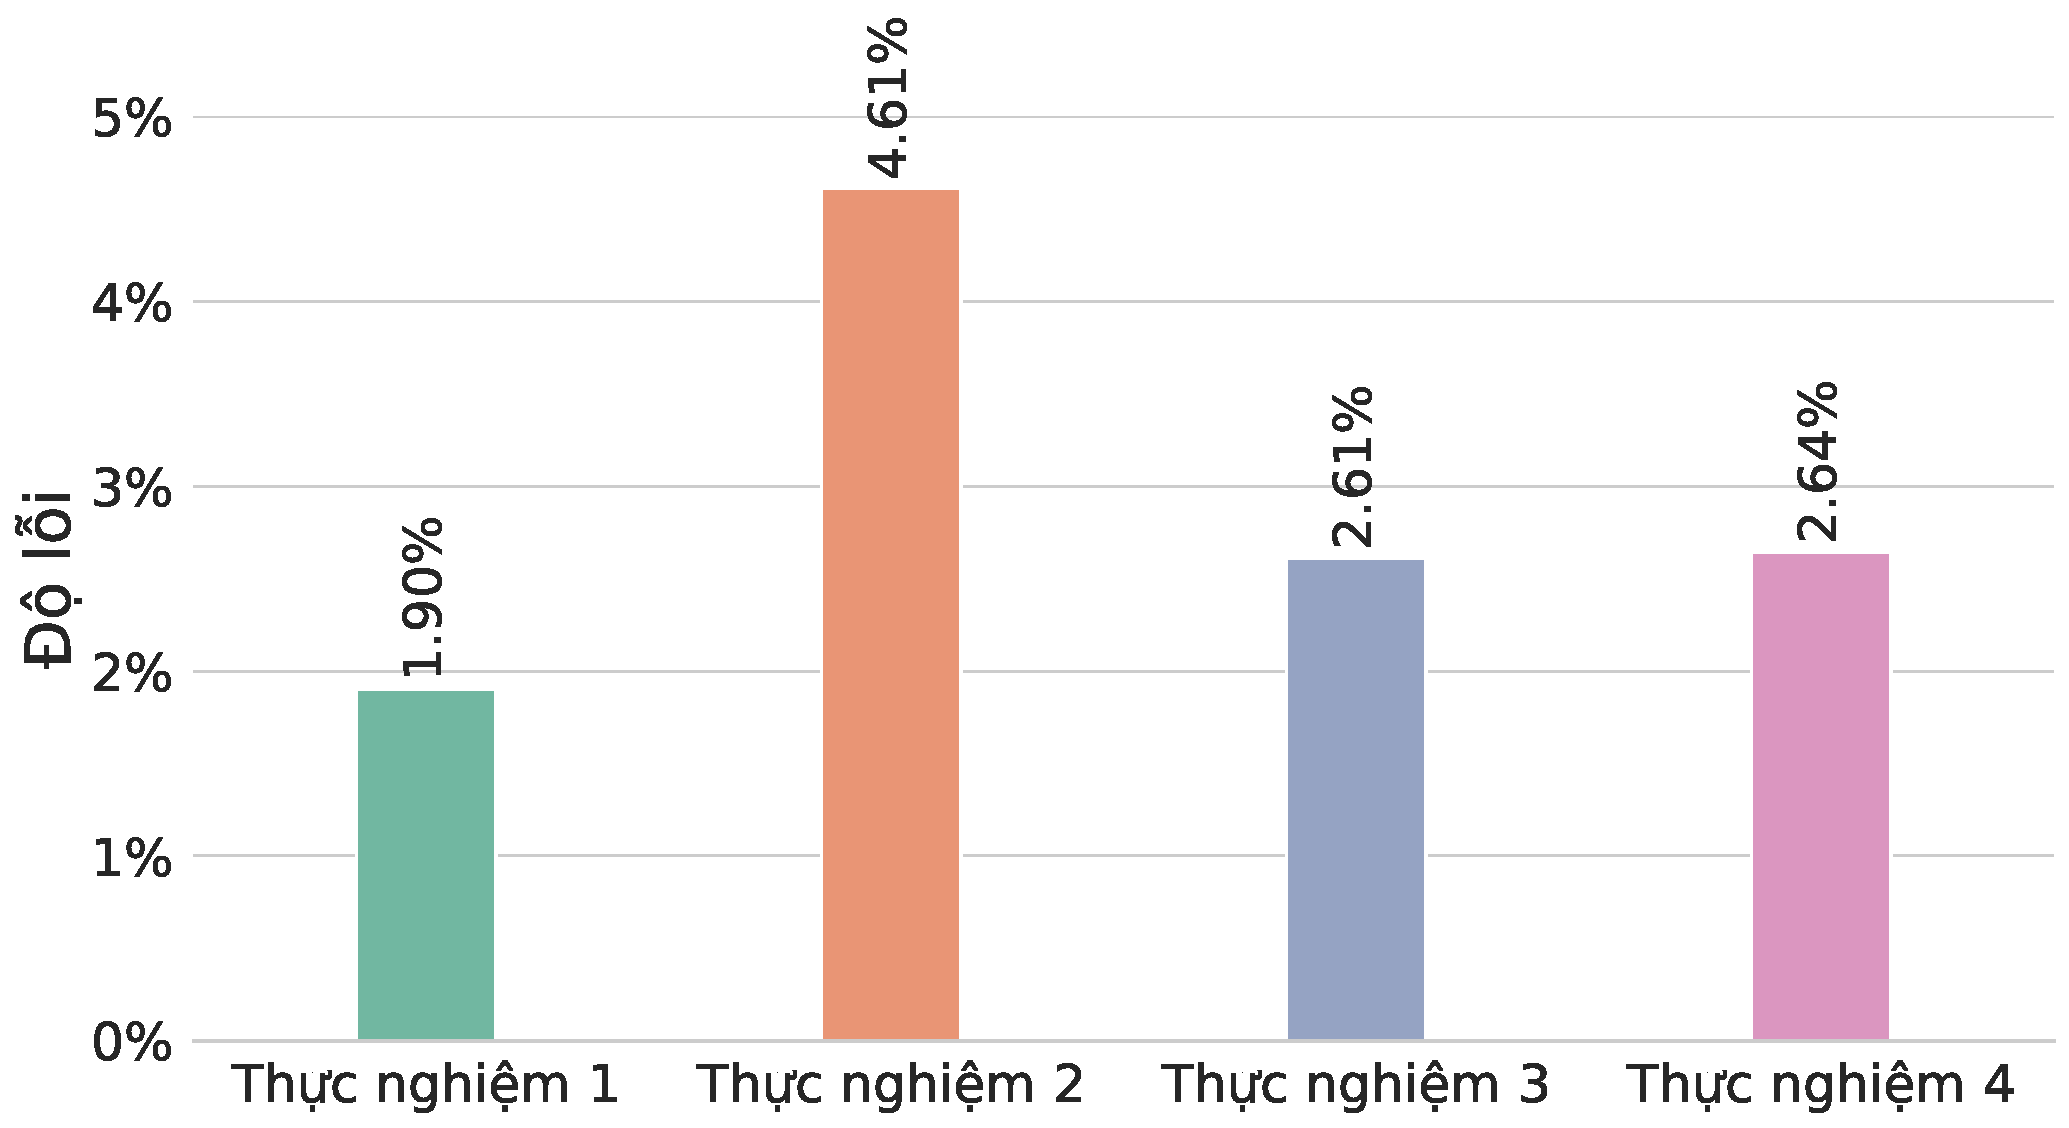
\includegraphics[width=\textwidth]{Figures/sensitive_error_rate.pdf}
    \caption[Minh họa tỷ lệ lỗi trung bình của các thí nghiệm ACO++ với các bộ siêu tham số khác nhau.]{Minh họa tỷ lệ lỗi trung bình từ mỗi thí nghiệm so với kết quả tốt nhất giữa bốn thí nghiệm cho mỗi nhóm trường hợp. Chúng tôi thực hiện 30 lần chạy độc lập cho mỗi trường hợp.}
    \label{fig:ACO++Sensitive}
\end{figure}

Kết quả của những thí nghiệm này được trình bày trong Hình \ref{fig:ACO++Sensitive}. Các thí nghiệm của chúng tôi cho thấy sự biến động đáng kể qua các bộ siêu tham số khác nhau cho thuật toán ACO++. Đặc biệt là sự chênh lệch đáng chú ý được quan sát trong Thí nghiệm 2, nơi việc hoán đổi các bộ tham số dẫn đến sự tăng đáng kể 4,61\% trong tỷ lệ lỗi - hơn gấp đôi con số của Thí nghiệm 1, nơi sử dụng cấu hình tham số cụ thể cho từng trường hợp, mang lại tỷ lệ lỗi chỉ là 1,90\%. Ngược lại, Thí nghiệm 3 và 4 thể hiện tỷ lệ lỗi tương đương khoảng 2,60\%. Các thí nghiệm của chúng tôi ở đây cho thấy sự nhạy cảm của ACO++ đối với các siêu tham số của nó.

\section{Cơ chế thích ứng tốc độ bay hơi pheromone}\label{section:AdaptivePheromoneRate}
Các thuật toán heuristics thường rất nhạy cảm đối với cài đặt tham số và do đó, chúng thiếu tính ổn định để giải quyết mọi cấu hình vấn đề một cách tổng quát. Vấn đề này thường được xử lý bằng cách sử dụng mỗi bộ tham số riêng cho từng trường hợp. Điều này rất tốn thời gian khi ta xem xét đến tính thực tế của thuật toán.

Từ quan điểm này, thì có vẻ như tham số quan trọng nhất đối với các thuật toán dựa trên tối ưu hóa đàn kiến là hệ số bay hơi mùi $\rho$. Hệ số này kiểm soát tốc độ bay hơi của pheromone, ảnh hưởng quyết định đến quá trình hội tụ của thuật toán. Giá trị càng lớn, quá trình hội tụ đến một điểm tối ưu cục bộ càng nhanh. Việc chọn giá trị bay hơi $\rho$ phù hợp phụ thuộc vào bản đồ mà trường hợp thuật toán đang giải.

Công trình về phương pháp AACO-NC \cite{STODOLA2022101056}, một thuật toán cho TSP, đã đề xuất một phương pháp thích ứng tham số tốc độ bay hơi pheromone $\rho$ cho thuật toán dựa trên tối ưu hóa đàn kiến. Ý tưởng của phương pháp này là tham số $\rho$ sẽ không cố định xuyên suốt quá trình thuật toán xử lý. Tham số $\rho$ sẽ thay đổi trong quá trình tối ưu hóa dựa trên thông tin đa dạng của các lời giải sinh ra bởi đàn kiến, thông tin này gọi là entropy. Tại điểm bắt đầu tối ưu hóa, khi mà độ đa dạng của lời giải đàn kiến lớn (giá trị entropy lớn) bởi vì các lời giải hoàn toàn ngẫu nhiên, thì giá trị của tốc độ bay hơi $\rho$ phải lớn để đảm bảo thuật toán hội tụ nhanh. Tuy nhiên, trong quá trình tối ưu hóa, khi mà các lời giải của đàn kiến bắt đầu hội tụ vào một điểm tối ưu cục bộ nào đó, giá trị tốc độ bay hơi $\rho$ nên giảm xuống để mở rộng không gian tìm kiếm.

Giá trị độ đa dạng của các lời giải trong đàn kiến được tính dựa trên công thức Shannon entropy H được trình bày bởi công thức dưới đây.

\begin{equation}\label{eq:AACO-NC:entropy}
    H = -\sum_{i=2}^{n}\sum_{j=1}^{i-1}p_{ij} \cdot \log_2 p_{ij}
\end{equation}

Trong đó $p_{ij}$ là xác suất mà cạnh $E_{ij}$ nối 2 đỉnh $v_i$ và $v_j$ ($i \neq j$) xuất hiện trong bất kỳ lời giải của đàn kiến. Giá trị xác suất này được tính bằng số lần xuất hiện của cạnh trong các lời giải theo công thức sau

\begin{equation}\label{eq:AACO-NC:entropy_prob}
    p_{ij} = \frac{\textit{\# số lần xuất hiện}(E_{ij})}{n \cdot n_{ants}}
\end{equation}

với $\textit{số lần xuất hiện}(E_{ij})$ là số lần cạnh $E_{ij}$ nối 2 đỉnh $v_i$ và $v_j$ xuất hiện trong các lời giải của đàn kiến.

Giá trị giới hạn cực tiểu và cực đại của entropy cho các lời giải của đàn kiến  được tính theo hai công thức \ref{eq:AACO-NC:entropymin} và \ref{eq:AACO-NC:entropymax}.

\begin{equation}\label{eq:AACO-NC:entropymin}
    H_{min} = \log_2 \frac{1}{n}
\end{equation}

\begin{equation}\label{eq:AACO-NC:entropymax}
    H_{min} = \log_2 \frac{1}{n\cdot n_{ants}}
\end{equation}

với n là số lượng đỉnh trong đồ thị (hay số lượng thành phố trong bản đồ); $n_{ants}$ là số lượng lời giải sinh ra bởi đàn kiến.

Tham số tốc độ bay hơi $\rho$ thay đổi trong khoảng giới hạn được gán tại thời điểm bắt đầu thuật toán:
\begin{itemize}
    \item $\rho_{min}$: cận dưới của tham số tốc độ bay hơi ($0 < \rho_{min} \leq \rho_{max}$)
    \item $\rho_{min}$: cận trên của tham số tốc độ bay hơi ($\rho_{min} \leq \rho_{max} < 1$)
\end{itemize}

Giá trị của tham số tốc độ bay hơi pheromone $\rho$ ở mỗi thế hệ được tính theo công thức \ref{eq:AACO-NC:adaptrho}. Công thức này thể hiện tham số $\rho$ phụ thuộc tuyến tính vào giá trị entropy giới hạn.

\begin{equation}\label{eq:AACO-NC:adaptrho}
    \rho = \rho_{\text{min}} + (\rho_{\text{max}} - \rho_{\text{min}}) \cdot \frac{H - H_{\text{min}}}{H_{\text{max}} - H_{\text{min}}}.
\end{equation}

Điểm mạnh của nguyên tắc này là tham số tốc độ bay hơi phản ánh sự tiến triển hiện tại trong quá trình tối ưu hóa. Khi quần thể có xu hướng hội tụ đến một tối ưu cục bộ, tham số cũng được giảm, do đó, pheromone bay hơi chậm hơn với ảnh hưởng của sự hội tụ chậm hơn. Điều này mở rộng không gian tìm kiếm dẫn đến khả năng khám phá một tối ưu cục bộ tốt hơn (hoắc có thể là toàn cục).

\section{Thuật toán tiến hóa CMA-ES}\label{section:bgCMA-ES}
Thuật toán Covariance Matrix Adaptation Evolution Strategy (CMA-ES) là một phương pháp tối ưu hóa tiến hóa được thiết kế để giải quyết các bài toán tối ưu hóa không đạo hàm. Được đề xuất bởi Nikolaus Hansen vào năm 2003 \cite{hansen2003ecj}, CMA-ES đã trở thành một trong những thuật toán quan trọng trong lĩnh vực tối ưu hóa tiến hóa.

CMA-ES kết hợp giữa hai yếu tố chính là ma trận hiệp phương sai (covariance matrix) và chiến lược tiến hóa (evolution strategy). Trong quá trình tối ưu hóa, thuật toán không chỉ tìm kiếm giải pháp tốt mà còn điều chỉnh ma trận hiệp phương sai để thích ứng với cấu trúc hình dạng của không gian tìm kiếm.

\begin{figure}[ht!]
    \centering
    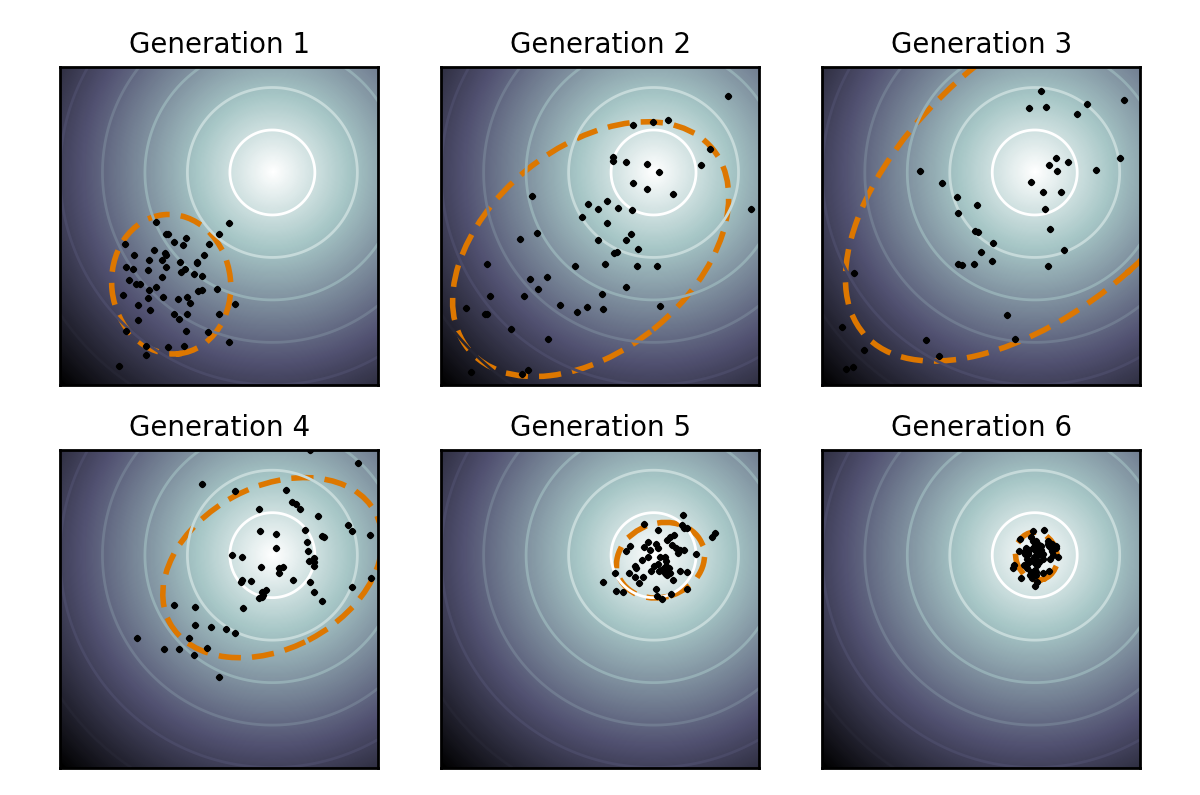
\includegraphics[width=0.85\textwidth]{Figures/Concept_of_directional_optimization_in_CMA-ES_algorithm.png}
    \caption[Minh họa quá trình CMA-ES tối ưu hóa một bài toán 2 chiều đơn giản.]{Minh họa quá trình CMA-ES tối ưu hóa một bài toán 2 chiều đơn giản. Địa hình tối ưu hóa hình cầu được biểu diễn dưới các đường liền. Quần thể được biểu diễn dưới các chấm và phân phối của CMA-ES được biểu diễn bằng đường đứt nét thay đổi qua các thế hệ. Trong bài toán đơn giản này, quần thể tập trung vào cực trị toàn cục chỉ trong vài thế hệ.}
    \label{fig:CMA-ES}
\end{figure}

Một đặc điểm nổi bật của CMA-ES là khả năng xử lý các bài toán tối ưu hóa không đạo hàm và không yêu cầu thông tin đạo hàm của hàm mục tiêu. Điều này làm cho nó trở thành lựa chọn phù hợp trong nhiều ứng dụng thực tế, khi mà việc tính toán đạo hàm có thể khó khăn hoặc tốn kém. Thuật toán thực hiện quá trình tối ưu hóa thông qua việc tạo ra và cập nhật một quần thể các cá thể (solutions) theo thời gian. Các cá thể này được tổ chức thành một phân phối xác suất, và chiến lược tiến hóa được sử dụng để điều chỉnh phân phối này sao cho các cá thể có khả năng sinh sản tốt nhất được ưu tiên. Với sự linh hoạt và hiệu suất của mình, CMA-ES đã được áp dụng rộng rãi trong nhiều lĩnh vực như tối ưu hóa tham số, máy học, và các ứng dụng trong khoa học dữ liệu.

Trong giải thuật \ref{algo:CMAES}, chúng tôi trình bày mã giả tóm tắt đầy đủ cho thuật toán CMA-ES. Giải thuật \ref{algo:CMAES} bắt đầu bằng cách khởi tạo các tham số ở dòng \ref{CMAES-algo:step1} là \ref{CMAES-algo:step2}. Các tham số của thuật toán bao gồm vị trí trung tâm của phân phối m, ma trận hiệp phương sai C, và bước nhảy $\sigma$. Ba tham số này {m, C, $\sigma$} sẽ được tuần tự cập nhật từ dòng \ref{CMAES-algo:step3} đến dòng \ref{CMAES-algo:step11} của thuật toán. Dòng \ref{CMAES-algo:step4} là lấy mẫu một quần thể  từ phân phối chuẩn với vị trí trung tâm m và hiệp phương sai C. Dòng \ref{CMAES-algo:step5} đánh giá các cá thể trong quần thể bằng một hàm hộp đen $f(.)$. Sau đó thuật toán sẽ dùng thông tin đánh giá này để cập nhật vị trí trung tâm m bằng cách lấy tổng $\mu$ cá thể tốt nhất ở dòng \ref{CMAES-algo:step6}, các trọng số được tính bằng log($\mu$/2) - log(i). Ký hiệu $y_{i:\lambda}$ nghĩa là các cá thể tốt nhất từ $y_i$, ..., $y_\lambda$. Ma trận hiệp phương sai được cập nhật ở dòng \ref{CMAES-algo:step10} bao gồm 3 phần: (1) thông tin cũ, (2) cập nhật bậc 1 (được tính bằng sự thay đổi của vị trí trung tâm hay còn gọi là đường tiến hóa $p_c$), và (1) cập nhật bậc $\mu$ được tính bằng các các thể tốt ở quần thể vừa rồi. Tham số bước nhảy được cập nhật ở dòng \ref{CMAES-algo:step8} dựa trên đường tiến hóa liên hợp $p_\sigma$. Mục tiêu của nó là tăng tốc tốc độ hội tụ vào cực trị, trong khi ngăn chặn việc hội tụ sớm. Các tham số khác bao gồm: $\mu_w$ là giá trị chọn hiệu quả phương sai, các tham số tốc độ học $c_1$, $c_c$, $c_\sigma$, và $d_\sigma$ là giá trị làm mượt cho $\sigma$. Các thông số của các tham số này được nghiên cứu kỹ lưỡng và thảo luận sâu trong \cite{hansen2023cma}. Điều kiện để kết thúc có thể được cài đặt nhiều cách khác nhau tùy thuộc vào không gian tìm kiếm, hoặc hàm thích nghi.

\begin{algorithm}
\caption{Thuật toán CMA-ES}
\label{algo:CMAES}
khởi tạo $\mathbf{m} \in \Re^n, \sigma \in \Re^{+}, \lambda, \mu$ \; \label{CMAES-algo:step1}
khởi tạo $\mathbf{C}=\mathbf{I}, \mathbf{p}_c=\mathbf{0}, \mathbf{p}_\sigma=\mathbf{0}$ \;\label{CMAES-algo:step2}
\Repeat{điều kiện dừng được thỏa mãn}{ \label{CMAES-algo:step3} 
lấy mẫu: $\theta_i=\mathbf{m}+\sigma \mathbf{y}_i, \mathbf{y}_i \sim \mathcal{N}(\mathbf{0}, \mathbf{C}), i=1, \ldots, \lambda$ \; \label{CMAES-algo:step4} 
đánh giá: $f\left(\theta_i\right), i=1, \ldots, \lambda$\; \label{CMAES-algo:step5} 
\tcp{cập nhật giá trị trung bình}
$\mathbf{m} \leftarrow \mathbf{m}+\sigma \overline{\mathbf{y}}$, với $\overline{\mathbf{y}}=\sum_1^\mu w_i \mathbf{y}_{i: \lambda}$\; \label{CMAES-algo:step6} 
\tcp{cập nhật bước nhảy}
$\mathbf{p}_\sigma \leftarrow\left(1-c_\sigma\right) \mathbf{p}_\sigma+\sqrt{c_\sigma\left(2-c_\sigma\right) \mu_w} \mathbf{C}^{-\frac{1}{2}} \overline{\mathbf{y}}$\; \label{CMAES-algo:step7} 
$\sigma \leftarrow \sigma \exp \left(\frac{c_\sigma}{d_\sigma}\left(\frac{\left\|\mathbf{p}_\sigma\right\|}{\mathbb{E}\|\mathcal{N}(\mathbf{0}, \mathbf{I})\|}-1\right)\right)$ \;\label{CMAES-algo:step8} 
\tcp{cập nhật ma trận hiệp phương sai}
$\mathbf{p}_c \leftarrow\left(1-c_c\right) \mathbf{p}_c+\sqrt{c_c\left(2-c_c\right) \mu_w} \overline{\mathbf{y}}$\;\label{CMAES-algo:step9} 
$\mathbf{C} \leftarrow\left(1-c_1-c_\mu\right) \mathbf{C}+c_1 \mathbf{p}_c \mathbf{p}_c^{\top}+c_\mu \sum_1^\mu w_i \mathbf{y}_{i: \lambda} \mathbf{y}_{i: \lambda}^{\top}$\;\label{CMAES-algo:step10} 
}\label{CMAES-algo:step11}
\end{algorithm}

\section{Kỹ thuật cài đặt tham số}\label{section:parametersetting}
Với các thuật toán heurisitic như thuật toán tối ưu hóa đàn kiến và thuật toán tiến hóa thì hiệu suất của các thuật toán này phụ thuộc phần lớn vào các tham số của chúng. Ở khóa luận này chúng tôi đặt trọng tâm vào việc tự động thích ứng các tham số của thuật toán ACO++, một thuật toán heuristic. Để dễ dàng nắm bắt được những kỹ thuật mà chúng tôi trình bày, ở phần này chúng tôi trình bày kiến thức cơ bản về các kỹ thuật cài đặt siêu tham số khác nhau cho một thuật toán heuristic.

Chúng tôi xem rằng có hai loại cài đặt tham số chính là điều chỉnh siêu tham số (parameter tuning) và kiểm soát siêu tham số (parameter control) \cite{771166}. Với điều chỉnh siêu tham số, là phương pháp cài đặt tham số thường xuyên được sử dụng, thì quá trình tìm ra các giá trị tham số tốt được thực hiện trước khi thuật toán chạy và sau đó dùng những tham số được tìm thấy cho thuật toán và không thay đổi trong quá trình chạy. Phương pháp điều chỉnh siêu tham số là hướng tiếp cận điển hình khi thiết kế thuật toán. Quá trình điều chỉnh được thực hiện bằng cách thử nghiệm nhiều giá trị tham số và chọn thủ công ra bộ tham số có kết quả tốt nhất. Tuy nhiên, với phương pháp này thì số lượng tham số và khoảng giá trị của chúng có thể dẫn đến quá trình điều chỉnh siêu tham số này rất tốn thời gian. Và phương pháp này có thể dẫn đến hiệu suất tổng quát thuật toán không tốt nếu các tham số này chỉ được thử nghiệm trên một tập trường hợp nhất định.

Phương pháp kiểm soát tham số là phương pháp đối nghịch với phương pháp điều chỉnh tham số trên. Các tham số sẽ được gán các giá trị khởi tạo khi bắt đầu thuật toán và thay đổi trong quá trình thuật toán chạy. Phương pháp này có thể giải quyết được vấn đề hiệu suất tổng quát của thuật toán bởi vì các tham số sẽ thay đổi giá trị theo từng trường hợp trong quá trình chạy của thuật toán. Hơn nữa với phương pháp này, nếu ta thiết kế nó đủ thông minh, nó có thể không cần tới quá trình điều chỉnh tham số thủ công tốn thời gian mà vẫn tìm ra tham số tốt cho thuật toán. Ở kỹ thuật kiểm soát tham số này, các tác giả của công trình \cite{771166} đã phân loại ra ba cơ chế con dựa trên cách hoạt động của chúng bao gồm cơ chế xác định, cơ chế thích ứng, cơ chế tự thích ứng. Hình \ref{fig:parameterSettingTaxonomy} Minh họa phân loại các kỹ thuật cài đặt tham số.

\begin{figure}[ht!]
    \centering
    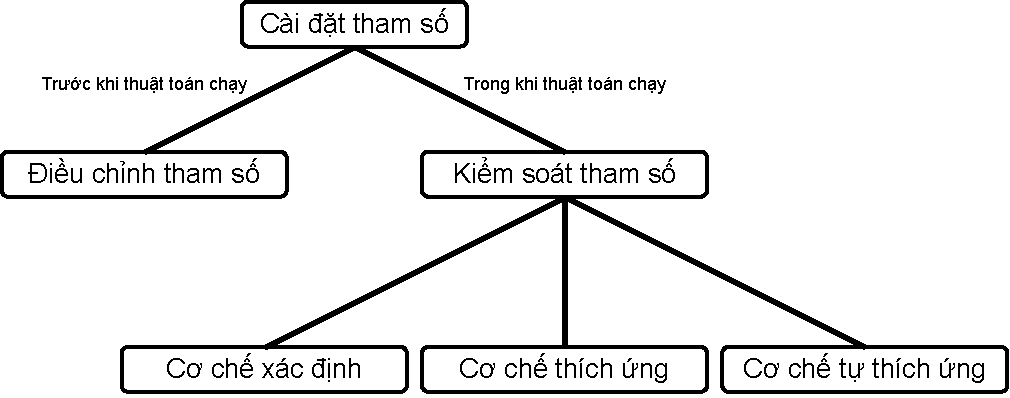
\includegraphics[width=0.8\textwidth]{Figures/Parameter setting.drawio.pdf}
    \caption[Minh họa phân loại các kỹ thuật cài đặt tham số.]{Minh họa phân loại các kỹ thuật cài đặt tham số}
    \label{fig:parameterSettingTaxonomy}
\end{figure}

Cơ chế kiểm soát tham số xác định là cơ chế mà khi giá trị của một tham số được thay đổi bởi một quy tắc xác định. Quy tắc này điều chỉnh tham số  theo một cách cố định, quy tắc xác định được định nghĩa sẵn (tức là được định nghĩa thủ công) mà không sử dụng bất kỳ phản hồi nào từ quá trình tìm kiếm. Thông thường, thì cơ chế này giống như cơ chế lập lịch mà tham số biến đổi theo thời gian.

Cơ chế kiểm soát tham số thích ứng là cơ chế mà khi có một hình thức phản hồi từ quá trình tìm kiếm được sử dụng làm đầu vào cho một một thủ tục để điều chỉnh tham số. Việc gán giá trị cho tham số  có thể dựa trên chất lượng của các lời giải được tìm ra bởi thuật toán. Ví dụ cho cơ chế này là cơ chế thích ứng tốc độ bay hơi pheromone chúng tôi đã trình bày ở phần \ref{section:AdaptivePheromoneRate}, tham số tốc độ bay hơi của thuật toán được điều chỉnh dựa trên chất lượng của các lời giải mà thuật toán tìm được ở vòng lặp hiện tại. 

Cuối cùng là cơ chế kiểm kiểm soát tự thích ứng, ví dụ điển hình cho cơ chế này là thuật toán CMA-ES mà chúng tôi đã trình bày ở phần \ref{section:CMAES}. Ở đây, các tham số cần được điều chỉnh được mã hóa vào các cá thể và trải qua quá trình đột biến và tái kết hợp. Các giá trị tốt hơn của các tham số được mã hóa này dẫn đến các cá thể tốt hơn, từ đó có khả năng cao hơn để sống sót, tạo ra con cái và do đó lan truyền những giá trị tham số tốt hơn này. Điều này là sự phân biệt quan trọng giữa các cơ chế thích ứng và cơ chế tự thích ứng: trong trường hợp tự thích ứng, các cơ chế cho việc gán điểm và cập nhật các tham số chiến lược khác nhau là hoàn toàn ngụ ý, tức là chúng là các toán tử lựa chọn và biến đổi của chu kỳ tiến hóa chính nó.

\section{Phương pháp phân cụm thứ bậc}\label{section:bgClusterTree}

Phân cụm thứ bậc là một kỹ thuật phân cụm nhằm xây dựng một cấu trúc cây của các cụm hay cây cụm thứ bậc. Cây cụm thứ bậc mang cấu trúc dữ liệu cây với mỗi nút là một cụm. Trong đó, tập điểm dữ liệu của một nút con là một phần trong tập điểm dữ liệu của nút ba mẹ. Phân cụm thứ bậc có thể giúp biểu hiện cấu trúc phân cấp tự nhiên có trong các điểm dữ liệu.

Phân cụm thứ bậc có hai loại là phân cụm phân chia (divisive clustering) và phân cụm hội tụ (agglomerative clustering) \cite{shetty2021hierarchical}. Phân chia là một phương pháp từ trên xuống bắt đầu với một cụm bao gồm tất cả các điểm dữ liệu. Nó chia các cụm thành các cụm con một cách tuần tự cho đến khi bản thân cụm là một điểm dữ liệu. Ngược lại, phân cụm hội tụ là một phương pháp từ dưới lên bắt đầu với mỗi điểm dữ liệu như một cụm đơn và sau đó hợp nhất các cụm gần nhau để tạo ra các cụm lớn hơn cho đến khi chỉ còn lại một cụm chứa tất cả các điểm dữ liệu. Cách phân chia hoặc hợp nhất các cụm phụ thuộc vào ứng dụng và đặc tính của dữ liệu. Do đó, phân cụm thứ bậc có nhiều biến thể và độ phức tạp không gian, thời gian khác nhau \cite{murtagh2012algorithms, murtagh2017algorithms}.

\chapter{THUẬT TOÁN ĐỀ XUẤT} \label{chapter:OurProposed}

Trong chương này, chúng tôi sẽ trình bày chi tiết về thuật toán mà chúng tôi đã đề xuất để giải quyết bài toán điều hướng thu thập (ThOP). Mục tiêu của thuật toán là đạt được hiệu suất cao và đồng thời có khả năng tự động thích ứng với các tham số mà không làm tăng độ phức tạp của thuật toán.

\section{Tổng quan thuật toán} \label{section:OverallAlgo}

\begin{figure}
    \centering
    \includesvg[inkscapelatex=false, width=\columnwidth]{Figures/SAAS-HC-v3.svg}
    \caption[Các cải tiến của SAAS so với ACO++.]{Các cải tiến của SAAS so với ACO++. Trong đó, \textcolor{blue}{màu xanh dương} thể hiện thành phần \textbf{mới}, \textcolor{green}{màu xanh lá} thể hiện sự \textbf{điều chỉnh} thành phần cũ và màu trắng thể hiện sự giữ nguyên thành phần cũ.}
    \label{fig:saas_flowchart}
\end{figure}

Thuật toán của chúng tôi được phát triển dựa trên nền tảng của thuật toán ACO++ đã được giới thiệu trước đó. Như chúng tôi đã mô tả trong phần kiến thức nền tảng, ACO++ là một biến thể của giải thuật đàn kiến MAX-MIN Ant System (MMAS). Tuy nhiên, một trong nhược điểm của ACO++ là yêu cầu sự đặt trước các siêu tham số trước khi thực hiện thuật toán. Điều này tạo ra một thách thức do ảnh hưởng lớn của các siêu tham số đối với kết quả của thuật toán.

Để khắc phục hạn chế này, chúng tôi đã thực hiện hai phương pháp. Đầu tiên, chúng tôi đã cải tiến thuật toán để tự động thích ứng các tham số trong quá trình hoạt động. Thứ hai, chúng tôi đã áp dụng hai kỹ thuật nhằm giảm độ phức tạp của thuật toán, từ đó nâng cao khả năng tìm kiếm lời giải tốt cho bài toán ThOP. Hình \ref{fig:saas_flowchart} cho thấy bức tranh toàn cảnh về các cải tiến của SAAS so với ACO++. Trong đó, màu xanh dương thể hiện thành phần mới, màu xanh lá thể hiện sự điều chỉnh thành phần cũ và màu trắng thể hiện sự giữ nguyên thành phần cũ. Mã giả của thuật toán được trình bày chi tiết trong Giải Thuật \ref{algo:SAAS}.

\begin{algorithm}
\caption{Thuật toán SAAS cho bài toán ThOP}
\label{algo:SAAS}
\algorithmfootnote{$\zeta(\pi)$ bỏ đi các thành phố không có vật phẩm được thu tập từ chiến lược thu thập $z$ từ $\pi$.}
$\pi^{best} \gets \varnothing, z^{best} \gets \varnothing $\; \label{SAAS:initsolution}
khởi tạo CMA-ES\; \label{SAAS:initES}
xây dựng cây cụm thứ bậc\; \label{SAAS:init_trees}
\Repeat{Điều kiện dừng được thỏa mãn} { \label{SAAS:mainloopstart}
    pop $\gets$ lấy mẫu một quần thể từ CMA-ES\; \label{SAAS:sampleSE}
    \ForEach{indv $\in$ pop}{ \label{SAAS:indvstart}
        $\alpha,\beta,\theta,\delta,\gamma,\rho_{\text{min}},\rho_{\text{max}}$ $\gets$ indv.genome\;\label{SAAS:genome}
        cập nhật $\rho$\ bằng phương trình \ref{eq:AACO-NC:adaptrho}\; 
        \label{SAAS:adapt_rho}
        % $\Pi \gets$ construct $n_{\text{indv}}$ routes using ants\; \label{SAAS:eachant}
        % \ForEach{route $\pi \in \Pi $}{ \label{SAAS:eachroute}
        \For{$i:= 1\ \textbf{to}\ n_{\text{indv}}$}{ \label{SAAS:eachant}
            $\pi \gets$ xây dựng tuyến đường bằng một con kiến\; \label{SAAS:conroute}
            $\pi' \gets$  thực hiện tìm kiếm địa phương trên tuyến đường $\pi$\; \label{SAAS:localsearch}
            $z \gets$ xây dựng chiến lược thu thập cho $\pi$\; \label{SAAS:packing}
            $z' \gets$ xây dựng chiến lược thu thập cho $\pi'$\; \label{SAAS:newpacking}
            \If{giá trị lợi nhuận của $z'$ cao hơn giá trị lợi nhuận của $z$}{ \label{SAAS:comaparecurrent}
                $\pi \gets \pi', z \gets z' $\; \label{SAAS:replacecurrent}
            }
            
            \If{giá trị lợi nhuận của $z$ cao hơn giá trị lợi nhuận của $z^{best}$}{ \label{SAAS:comaparebest}
                $\pi^{best} \gets \zeta(\pi), z^{best} \gets z $\; \label{SAAS:replacebest}
            }\label{SAAS:comaparebestend}
        }

        indv.fitness $\gets$ giá trị lợi nhuận cao nhất trong các lời giải của quần thể\; \label{SAAS:indvfitness}
    } \label{SAAS:indvend}

    cập nhật tham số của CMA-ES \; \label{SAAS:updateES}
    \If{điều kiện khởi động lại CMA-ES được thỏa mãn}{ \label{SAAS:checkES} 
        khởi động lại CMA-ES\; \label{SAAS:restartES}
    }
    tính giá trị độ đa dạng lợi nhuận bằng công thức \ref{eq:entropy} và \ref{eq:entropy_prob}\; \label{SAAS:entropy}
    cập nhật $n_{\text{indv}}$ bằng công thức \ref{eq:adaptants}\; \label{SAAS:adapt_n_ant}
    cập nhật dấu vết của pheromone và số liệu của MMAS\; \label{SAAS:updatepheromone} 
}\label{SAAS:mainloopend}
\Return{$\pi^{best}, z^{best}$}\; \label{SAAS:return}
\end{algorithm}

Khi bắt đầu, thuật toán khởi tạo lời giải tốt nhất bằng một lời giải trống với một tuyến đường và một chiến lược thu thập (dòng \ref{SAAS:initsolution}). Các tham số của cơ chế tự thích ứng của CMA-ES cũng được khởi tạo (dòng \ref{SAAS:initES}). Đồng thời các cây cụm thứ bậc cho từng thành phố cũng được khởi tạo (dòng \ref{SAAS:init_trees}). Theo sau đó thuật toán vào vòng lặp chính (dòng \ref{SAAS:mainloopstart}), và vòng lặp này tiếp tục lặp lại cho đến khi điều kiện kết thúc được thỏa mãn (dòng \ref{SAAS:mainloopend}). Điều kiện để kết thúc vòng lặp là khi thời gian thuật toán tìm kiếm vượt quá thời gian giới hạn của trường hợp đang xét.

Tại vòng lặp chính (dòng \ref{SAAS:mainloopstart} đến dòng \ref{SAAS:mainloopend}), đầu tiên thuật toán lấy mẫu một quần thể từ cơ chế tự thích ứng của CMA-ES (dòng \ref{SAAS:sampleSE}). Với mỗi cá thể trong quần thể vừa được lấy mẫu (từ dòng \ref{SAAS:indvstart} đến dòng \ref{SAAS:indvend}), một tập con của đàn kiến tìm kiếm một tập các lời giải bằng cách sử dụng các tham số được lấy từ thông tin của mỗi cá thể (dòng \ref{SAAS:genome}). 

Với mỗi con kiến tập con đó (dòng \ref{SAAS:eachant}), nó sẽ khám phá ra một tuyến đường $\pi$ dựa trên thông tin dấu vết pheromone (dòng \ref{SAAS:conroute}. Sau đó thuật toán tạo ra một tuyến đường khác $\pi^{'}$ từ tuyền đường vừa tìm được với con kiến với độ dài được thử để giảm quãng đường bằng phương pháp tìm kiếm địa phương 2-OPT\cite{Crama1995}. Tiếp theo, thuật toán sử dụng phương pháp thu thập vật phẩm để sinh ra chiến lược thu tập cho hai tuyền đường đó (dòng \ref{SAAS:packing} và \ref{SAAS:newpacking}). Nếu lợi nhuận của chiến lược thu thập của tuyến đường đường cải thiện $\pi^{'}$ tốt hơn tuyến đường gốc $\pi^{'}$ thì thay thế tuyến đường gốc và chiến lược thu thập bằng tuyến đường được cải thiện và chiến lược thu thập của nó (dòng \ref{SAAS:comaparecurrent}). Sau đó cập nhật lời giải tốt nhất bằng cách so sánh với lời giải hiện tại (dòng \ref{SAAS:comaparebest}).

Phương pháp thu thập vật phẩm của thuật toán chúng tôi giống với phương pháp được sử dụng trong thuật toán ACO++\cite{Chagas2021}. Tuy nhiên chúng tôi đã chỉnh sửa các giá trị tham số của $\theta$, $\delta$, và $\gamma$ không cần phải sinh bằng hàm ngẫu nhiên đồng nhất mà lấy từ thông tin của mỗi cá thể. Vậy nên thuật toán chúng tôi chỉ gọi hàm sinh ra chiến lược thu thập vật phẩm này một lần thay vì nhiều lần như thuật toán ACO++. Bởi vì CMA-ES của thuật toán chúng tôi có khả năng tự học để cải thiện các tham số này qua các cá thể của quần thể, trong khi trong thuật toán ACO++ cần gọi nhiều lần để tăng khả năng hàm sinh giá trị ngẫu nhiên sinh ra các giá trị tham số $\theta$, $\delta$, và $\gamma$ tốt cho phương pháp thu thập tham lam.

Giá trị sinh tồn của mỗi cá thể (giá trị indv.fitness) được quyết định bằng giá trị lợi nhuận (giá trị hàm mục tiêu) cao nhất của tập đàn kiến con sử dụng thông tin di truyền của nó để sinh ra các lời giải (dòng \ref{SAAS:indvfitness}). Khi tất cả các cá thể trong quần thể của CMA-ES đã tính xong giá trị sinh tồn của chúng, cơ chế tự thích ứng CMA-ES sử dụng các thông tin này để cập nhật học và cập nhật các tham số của nó để ở vòng lặp tiếp theo cơ chế sẽ sinh ra quần thể có các cá thể tốt hơn (dòng \ref{SAAS:updateES}). Nếu các tham số của CMA-ES chạm điều kiện khởi động lại thì cơ chế tự thích ứng CMA-ES sẽ khởi tạo lại các tham số của nó (dòng \ref{SAAS:restartES}). Chi tiết về cách cơ chế tự thích ứng CMA-ES hoạt động được trình bày ở phần \ref{section:CMAES}. 

Thuật toán sau đó tính giá trị đa dạng lợi nhuận của đàn kiến (Line \ref{SAAS:entropy}) của cơ chế thích ứng để điều chỉnh số lượng kiến ở trong mỗi đàn kiến con và giá trị bay hơi của pheromone (dòng \ref{SAAS:adapt_rho}). Chi tiết về cơ chế thích ứng này được trình bày ở phần \ref{section:ProfitAdaptive}. Ở cuối mỗi vòng lặp chính, thuật toán cập nhật dấu vết pheromone and các số liệu của phương pháp MMAS (dòng \ref{SAAS:updatepheromone}).

Lưu ý rằng chúng tôi đã thay thế cơ chế bay hơi của MMAS bằng cơ chế bay hơi lười biến ở những lúc thuật toán sử dụng thông tin dấu vết bay hơi (dòng \ref{SAAS:eachant} và dòng \ref{SAAS:updatepheromone}). Cơ chế bay hơi lười biến được trình bày chi tiết ở phần \ref{section:LazyEvaporation}. Ngoài ra khi mỗi con kiến tìm tuyến đường di chuyển (dòng \ref{SAAS:eachant}), đàn kiến trong giải thuật của chúng tôi di chuyển trên các cạnh của cây cụm thứ bậc, thay vì di chuyển trên các cạnh nối giữa các thành phố. Các thông tin dấu vết pheromone cũng được lưu và cập nhật trên các cạnh của cây. Mô tả và cách hoạt động của Kiến di chuyển trên cây cụm thứ bậc được trình bày ở phần \ref{section:AntTraversalClusterTrees}

Thuật toán sẽ tiếp tục lặp lại vòng lặp chính để cải thiện lời giải tốt nhất và giá trị của các tham số cho đên khi điều kiện dừng được thỏa mãn. Sau khi kết thúc vòng lặp chính thuật toán của chúng tôi trả về lời giải hiệu quả bao gồm tuyến đường cùng với chiến lược thu thập vật phẩm.


\section{Tận dụng thông tin sự đa dạng lợi nhuận cho cơ chế thích ứng}\label{section:ProfitAdaptive}

Cơ chế kiểm soát tham số đầu tiên chúng tôi cài đặt trong SAAS là cơ chế dựa trên giá trị lợi nhuận của các lời giải được tìm bởi đàn kiến. Cơ chế này được chúng tôi dựa vào cơ chế thích nghi của thuật toán AACO-NC\cite{STODOLA2022101056}, được trình bày ở phần \ref{section:AdaptivePheromoneRate}. Cơ chế của chúng tôi khác với của thuật toán AACO-NC ở hai điểm. Thứ nhất, cơ chế của chúng tôi thích ứng không chỉ tham số tốc độ bay hơi pheromone $\rho$ mà còn cho lượng kiến cho mỗi cá thể $n_{indv}$ của quần thể CMA-ES. Cũng giống như tham số $\rho$, số lượng kiến cho mỗi cá thể $n_{indv}$ đóng vai trò quan trọng việc cân bằng giữa khám phá và khai phá không gian tìm kiếm của thuật toán. 

Điểm khác biệt thứ hai là cơ chế của chúng tôi sử dụng giá trị lợi nhuận của các lời giải được tìm bởi đàn kiến ở vòng lặp hiện tại để thích ứng hai tham số trên. Khác với thuật toán AACO-NC giải quyết bài toán TSP, độ đa dạng của đàn kiến thể hiện qua sự khác nhau giữa các cạnh trong chu trình của lời giải, bài toán ThOP bao gồm hai cần tuyến đường và chiến lược thu thập nên chúng tôi chọn giá trị lợi nhuận của mỗi lời giải để tính độ đa dạng bởi vì nó đại diện cho cả hai thành phần này. Bởi vì sự khác biệt này nên chúng tôi đã chỉnh sửa lại các công thức của thuật toán AACO-NC.


Ở cuối mỗi vòng lặp chính, thuật toán của chúng tôi sẽ tính thông tin sự đa dạng lợi nhuận entropy $H$ bằng các lời giải trong đàn kiến bằng công thức Shannon entropy dưới đây:

\begin{equation}\label{eq:entropy}
\begin{split}
    S &= \{P\  |\ \text{$P$ là giá trị lợi nhuận của một lời giải được tìm thấy bởi đàn kiến hiện tại}\} ,\\
    H &= -\sum_{i=1}^{|S|} p_{i} \cdot \log_2 p_{i}
\end{split}
\end{equation}

Trong đó $p_{i}$ là xác suất của giá trị $P_i$, giá trị lợi nhuận thứ $i$ trong tập giá trị lợi nhuận $S$ được tìm thấy bởi đàn kiến. Xác suất này là tần suất xuất hiện của giá trị lợi nhuận $P_i$ trong tập lời giải được tìm bời đàn kiến:
\begin{equation}\label{eq:entropy_prob}
    p_{i} = \frac{\text{\# số lần xuất hiện}(P_{i})}{n_{\text{ants}}}
\end{equation}

Trong đó $n_{\text{ants}}$ là số con kiến trong đàn. Phạm vi giá trị entropy được giới hạn bởi $H_{\text{min}}$ và $H_{\text{max}}$:
\begin{equation}\label{eq:limit_entropy}
   H_{\text{min}} = -\log_2\frac{n_{\text{ants}}}{n_{\text{ants}}} = 0, \quad
   H_{\text{max}} = -\log_2\frac{1}{n_{\text{ants}}} .
\end{equation}

Tỷ lệ bay hơi pheromone $\rho$ được điều chỉnh theo công thức \ref{eq:AACO-NC:adaptrho} của thuật toán AACO-NC được trình bày ở phần \ref{section:AdaptivePheromoneRate}. Tương tự, với số lượng kiến mỗi cho cá thể $n_{indv}$ chúng tôi sử dụng một phiên bản sửa đổi của công thức \ref{eq:AACO-NC:adaptrho}:

\begin{equation} \label{eq:adaptants}
    n_{\text{indv}} = n_{\text{indv\_max}} - (n_{\text{indv\_max}} - n_{\text{indv\_min}}) \cdot \frac{H - H_{\text{min}}}{H_{\text{max}} - H_{\text{min}}}.
\end{equation}

Ở đây, số lượng kiến được gán cho mỗi cá thể, ký hiệu là $n_{\text{indv}}$, là cố định cho tất cả các cá thể. $n_{\text{indv\_max}}$ và $n_{\text{indv\_min}}$ là là  tham số đại diện cho giới hạn lớn nhất và nhỏ nhất của số lượng kiến cho mỗi cá thể. Khác với tham số tốc độ bay hơi $\rho$, giá trị của $n_{\text{indv}}$ tăng khi sự đa dạng lợi nhuận thấp để khuyến khích khám phá và giảm khi đa dạng cao để tăng cường khai phá không gian tìm kiếm. Sự tích hợp thông tin sự đa dạng lợi nhuận cải thiện chiến lược thích ứng, tạo ra sự cân bằng giữa khám phá và khai thác.

\section{Cơ chế tự thích ứng sử dụng CMA-ES}\label{section:CMAES}

Thuật toán ACO++ được tác giả điều chỉnh các siêu tham số riêng cho từng nhóm trường hợp để cải thiện tính ổn định của hiệu suất thuật toán. Chúng tôi đề xuất tích hợp một cơ chế tự thích ứng để điều chỉnh các tham số trong quá trình tìm kiếm lời giải của thuật toán. Một số tham số có thể tự thích ứng được liệt kê trong bảng \ref{tab:control_param}. Cơ chế này cho phép các tham số thích nghi với đặc điểm riêng biệt của trường hợp và quá trình tìm kiếm.

\begin{table}[ht!]
    \begin{center}
        \begin{tabular}{lcl}
            \toprule
            Tham số            &   Cơ chế kiểm soát tham số  & Khoảng giá trị \\
            \midrule
            $\alpha$                    &   Tự thích ứng   & [0, 1]\\
            $\beta$                     &   Tự thích ứng  & [0, 1]     \\
            $\rho_{\text{min}}$, $\rho_{\text{max}}$  &   Tự thích ứng & [0, 1] \\
            $\theta$                    &   Tự thích ứng & [0, 1]             \\
            $\delta$                    &   Tự thích ứng & [0, 1]             \\
            $\gamma$                    &   Tự thích ứng & [0, 1]             \\
            $n_{\text{indv}}$           &   Thích ứng       & [$n_{\text{indv\_max}}$, $n_{\text{indv\_min}}$]  \\
            $\rho$                      &   Thích ứng         & [$\rho_{\text{min}}, \rho_\text{{max}}$] \\
            \bottomrule
        \end{tabular}
        \caption[Danh sách các tham số được kiểm soát bằng các kỹ thuật kiểm soát tham số]{\label{tab:control_param}Danh sách các tham số được kiểm soát bằng hai kỹ thuật kiểm soát tham số tự thích ứng và thích ứng}
    \end{center}
\end{table}

Tham số $\alpha$ và $\beta$ là hai tham số kiểm soát tính quan trọng của nồng độ pheromone và thông tin heuristic trong công thức tính xác suất di chuyển (công thức \ref{eq:ACOpheromone}). Tham số $\rho_{\text{min}}$ và $\rho_{\text{max}}$ là các tham số thể hiện cận trên là cận dưới cho tham số tốc độ bay hơi $\rho$, giúp cho cơ chế kiểm soát tham số thích ứng mà chúng tôi đã trình bày ở phần \ref{section:ProfitAdaptive}. Các tham số $\theta$, $\delta$, và $\gamma$, là các tham số điều chỉnh mức độ ảnh hưởng của các giá trị lợi nhuận, trọng lượng và khoảng cách trong công thức tính điểm của vật phẩm trong phương pháp thu thập heuristic (Công thức \ref{eq:itemScore}). Thuật toán CMA-ES sẽ kiểm soát các giá trị của tham số này qua một phân mối chuẩn đa biến. Phân phối chuẩn này được khởi tạo qua các giá trị trung tậm mặc định và giá trị bước nhảy mặc định cho từng tham số.

Trong phương pháp SAAS, chúng tôi sử dụng thuật toán CMA-ES để làm cơ chế tự thích ứng. Ở đầu mỗi lần lặp chính (Dòng \ref{SAAS:mainloopstart} đến Dòng \ref{SAAS:mainloopend}), một quần thể các bộ tham số được lấy mẫu từ CMA-ES. Sau đó, đối với mỗi cá thể trong quần thể này, một nhóm kiến con sẽ sử dụng các tham số đã được mã hóa trên cá thể đó để xây dựng các lời giải. Giá trị sinh tồn của mỗi cá thể được xác định bằng giá trị lợi nhuận cao nhất đạt được trong nhóm kiến con tương ứng của  cá thể đó. Sau khi giá trị sinh tồn cho tất cả các cá thể đã được tính, thuật toán CMA-ES sẽ điều chỉnh phân phối của nó để cái thiện khả năng sinh ra các cá thể tốt hơn ở dựa theo các bộ tham số có khả năng đạt được giá trị lợi nhuận cao hơn.

Để tránh thuật toán bị kẹt trong cực trị địa phương hoặc quá trình tìm kiếm không hiệu quả, chúng tôi đã cài đặt cơ chế khởi động lại cho CMA-ES, cơ chế mà sẽ gán lại phân phối của CMA-ES. Cơ chế này được kích hoạt khi mà giá trị bước nhảy trở nên quá nhỏ (đã hội tụ vào một cực trị địa phương) hoặc trở nên quá lớn vượt quá giới hạn của không gian tìm kiếm (quá trình tìm kiếm không hiệu quả).

\section{Kiến di chuyển trên cây cụm thứ bậc}\label{section:AntTraversalClusterTrees}
Với giải thuật đàn kiến thông thường, khi kiến cân nhắc di chuyển đến thành phố tiếp theo, chúng ta cần xem xét $n$ thành phố và tính xác suất dịch chuyển. Cách thức này có độ phức tạp về thời gian là $O(n)$. Nhận thấy kĩ thuật từ AACO-NC \cite{STODOLA2022101056} giúp giảm chi ở quá trình này. Cụ thể như sau, nếu ta cluster $n$ thành phố thành $k$ cụm, khi chọn thành phố tiếp theo, ta sẽ chọn cụm trước, rồi mới cân nhắc $n_\mathrm{size}$ thành phố trong cụm đó. Kĩ thuật này đã giúp giảm độ phức tạp xuống còn $O(k + n_\mathrm{size})$.

Khi được biết qua kĩ thuật trên, chúng tôi nhận thấy rằng nếu ta có thể giảm chi phí chọn thành phố bằng cách phân cụm chúng, vậy thì, tương tự, ta cũng có thể giảm chi phí chọn cụm bằng cách phân cụm chúng lần nữa và nhiều lần nữa. Chúng tôi quyết định xây dựng cây cụm thứ bậc, nơi mà các nút con là các cụm được phân cụm từ nút ba mẹ. Nút gốc đại diện cho một cụm chứa tất cả thành phố, các nút lá đại diện cho các cụm chứa đúng một thành phố. Bằng cách duyệt cây từ gốc đến lá, ở mỗi nút, kiến sẽ cân nhắc $k$ cụm (nút) con, khi ấy chi phí chọn thành phố tiếp theo sẽ là $\Theta(k \cdot \log_{k} n)$.

Để tìm ra giá trị $k$ mang lại chi phí thấp nhất, chúng tôi gọi
\begin{align*}
    f(k) &= k \cdot \log_{k} n \\
    &= \ln n \cdot \frac{k}{\ln k}
\end{align*}
và tiến hành tìm cực trị của hàm f:
\begin{align*}
    &\text{Xét } f'(k) = 0 \\
    \Leftrightarrow& \ln n \cdot \frac{\ln k -1 }{\ln^2  k} = 0\\
    \Rightarrow& \ln k - 1 = 0 \\
    \Leftrightarrow&\ k = \mathrm{e}.
\end{align*}
\begin{figure}
    \centering
    \includesvg[inkscapelatex=false, width=0.75\columnwidth]{Figures/k_value.svg} \\
    \caption{Ảnh hưởng của $k$ đến chi phí chọn thành phố tiếp theo.}
    \label{fig:k_value}
\end{figure}
Nhìn hình \ref{fig:k_value}, ta có thể thấy 2 và 3 là hai giá trị nguyên gần với e nhất và $f(3) < f(2)$. Do đó chọn $k$ bằng 3 sẽ mang lại chi phí tốt nhất. Tuy vậy, trong quá trình thực nghiệm, chúng tôi đã chọn $k$ bằng 2. Khi giá trị $k$ được cố định, độ phức tạp về thời gian của việc chọn thành phố tiếp theo sẽ là $\Theta(\log n).$

Chúng tôi xác định sáu đặc trưng cho mỗi thành phố để tiến hành phân cụm. Các đặc trưng bao gồm toạ độ x, tọa độ y của thành phố, khoảng tin cậy  của trọng lượng và lợi nhuận của các vật phẩm thuộc thành phố. Thông tin về trọng lượng và lợi nhuận sẽ có khoảng tin cậy riêng và mỗi khoảng tin cậy tương ứng với 2 đặc trưng. Cụ thể, đầu tiên, ta tính giá trị trung bình mean và độ lệch chuẩn std từ các vật phẩm trong thành phố. Sau đó, ta chọn biên dưới $\mathrm{mean} - 2 \cdot \mathrm{std}$ và biên trên $\mathrm{mean} + 2 \cdot \mathrm{std}$ của khoảng tin cậy để làm đặc trưng. Việc thêm thông tin vật phẩm vào đặc trưng giúp ta phân cụm các thành phố có cùng phân bố vật phẩm. Từ đó giúp đàn kiến khám phá các thành phố lân cận hiệu quả hơn.

Thành phố bắt đầu là nơi chỉ có thể rời khỏi, không thể đi tới, do đó, nó không cần thêm vào cây cụm thứ bậc. Mặt khác, thành phố kết thúc, nơi mà không có vật phẩm nào, nghĩa là nó không thể có đặc trưng cho vật phẩm, do đó nó cần được phân cụm theo cách riêng. Cụ thể, ở lớp đầu tiên ngay dưới nút gốc, ta thủ công phân cụm thành phố kết thúc thành một cụm riêng và các thành phố còn lại thành một cụm. Đối với các thành phố khác, chúng tôi sử dụng phương pháp phân cụm thứ bậc phân chia (divisive hierarchical clustering) với K-Means làm phương pháp tách (Hình \ref{fig:hc_k-means}) để xây dựng cấu trúc cây.
\begin{figure}
    \centering
    \includesvg[inkscapelatex=false, width=1\columnwidth]{Figures/HC_K-Means.svg} \\
    \caption{Phân cụm thứ bậc phân chia (divisive hierarchical clustering) với K-Means làm phương pháp tách.}
    \label{fig:hc_k-means}
\end{figure}

Thuật toán phân cụm này là một cách hiệu quả để xây dựng cấu trúc cây cụm thứ bậc. Độ phức tạp về thời gian của phân cụm K-Means là $O(n \cdot t \cdot k \cdot d)$, trong đó $n$ là số lượng thành phố (hay số điểm dữ liệu) cần phân cụm, $t$ là số vòng lặp trong quá trình phân cụm, $k$ thể hiện số cụm và d thể hiện số đặc trưng của thành phố (hay số chiều của điểm dữ liệu). Giữa lớp của cây, mặc dù có số lượng nút khác nhau, và mỗi nút đại diện cho một lượng thành phố khác nhau, nhưng trong một lớp, tổng số thành phố không thể vượt quá $n$. Do đó, việc áp dụng K-Means tại một lớp của cậy để tạo ra một lớp mới sẽ tốn tổng chi phí là $O(n \cdot t \cdot k \cdot d)$. Vì mỗi nút có k nút con, nên cây có trung bình $\log_k n$ lớp, chi phí của thuật toán sẽ là $\Theta(\log_k n \cdot n \cdot t \cdot k \cdot d)$. Do $k$ và $d$ sẽ được mang giá trị cố định và không có liên hệ đến input, độ phức tạp về thời gian của việc xây dựng cấu trúc cây là $\Theta(n \cdot \log n \cdot t)$.

Trong phương pháp của chúng tôi, kiến sẽ di chuyển qua cây cụm thứ bậc thay vì di chuyển trực tiếp từ thành phố này sang thành phố khác. Mỗi thành phố có cây cụm thứ bậc riêng thể hiện các cạnh đi đến n thành phố và có chung một cấu trúc. Việc có cấu trúc cây giống hệt nhau ở mọi thành phố cho phép thuật toán đánh dấu hiệu quả thành phố nào đã được được đi qua.

Ngược lại với AACO-NC, chúng tôi sử dụng pheromone và heuristic riêng biệt cho các cạnh của cây để tính toán xác suất chuyển đổi. Heuristic của một cạnh trên cây được định nghĩa là khoảng cách từ thành phố hiện tại đến tọa độ trọng tâm của cụm đích.

Trong các cây không cân bằng, lá ở độ sâu nông hơn thường có xác suất được chọn cao hơn. Để giải quyết vấn đề này, chúng tôi điều chỉnh trọng số chuyển đổi đến một nút con bằng cách nhân nó với số lượng lá dưới nút con đó. Điều này có nghĩa là trọng số chuyển đổi sang một nút, lúc này, mang tính đại diện cho tổng trọng số chuyển đổi đến các lá của nó.

\section{Bay hơi lười biếng}\label{section:LazyEvaporation}

Ở các giải thuật đàn kiến khác, việc bay hơi pheromone thường được thực hiện bằng cách duyệt qua từng cạnh trên bản đồ và nhân nồng độ pheromone của cạnh với $(1-\rho)$, mang độ phức tạp thời gian $O(n^2)$. Cách này tương đối lãng phí bởi vì phần lớn các cạnh ít khi được kiến đi qua, ta điều chỉnh dấu vết pheromone mà chưa thực sự dùng đến. Để khắc phục nhược điểm trên, chúng tôi đề xuất kỹ thuật Bay hơi lười biếng giúp thuật toán đạt được hiệu quả bay hơi tương tự với độ phức tạp thấp hơn. Bay hơi lười biếng giảm độ phức tạp bằng cách trì hoãn cập nhật các vết pheromone chưa dùng đến.

Nguyên tắc cốt lõi của bay hơi lười biếng là theo dõi trạng thái mong muốn và trạng thái lịch sử. Trạng thái mong muốn bao gồm hai biến DECount và DRCount. DECount theo dõi số lần bay hơi (mong muốn) kể từ lần cuối (mong muốn) khởi tạo lại pheromone. DRCount theo dõi số lần (mong muốn) khởi tạo lại pheromone kề từ lúc thuật toán bắt đầu. Ứng với mỗi cạnh là một trạng thái lịch sử riêng, bao gồm $\tau_{\text{historical}}$, HECount và HRCount. $\tau_{\text{historical}}$ là nồng độ pheromone lịch sử của cạnh tương ứng tại thời điểm HECount và HRCount. HRCount ghi nhận số lần $\tau_{\text{historical}}$ đã khởi tạo lại. HECount ghi nhận số lần $\tau_{\text{historical}}$ đã bay hơi kể từ lần khởi tạo lại pheromone thứ HRCount.

Bằng cách so sánh trạng thái lịch sử và trạng thái mong muốn, chúng ta có thể xác định nồng độ pheromone mong muốn $\tau_{\text{desired}}$ cho các cạnh cần dùng đến. Nếu HRCount nhỏ hơn DRCount, có nghĩa là cạnh chưa được cập nhật kể từ lần khởi tạo lại pheromone trước đó, vì vậy thuật toán sẽ đặt lại $\tau_{\text{historical}}$ bằng pheromone khởi tạo lại. Sau đó, $\tau_{\text{historical}}$ của cạnh được bay hơi (DECount - HECount) lần:
\begin{equation} \label{eq:lazy_evap}
    \tau_{\text{desired}} \gets \tau_{\text{historical}} \cdot (1 - \rho) ^ {\text{DECount} - \text{HECount}}.
\end{equation}

Bay hơi lười biếng trì hoãn điều chỉnh nồng độ pheromone khi giải thuật đàn kiến có mong muốn thực hiện bay hơi hoặc khởi tạo lại, thay vào đó, ta cập nhật trạng thái mong muốn. Trước khi tính xác suất chuyển tiếp, Bay hơi lười biếng sẽ khôi phục $\tau_{\text{desired}}$ bằng cách quan sát trạng thái mong muốn và trạng thái lịch sử. Khi cần rải thêm pheromone, ta đồng bộ trạng thái lịch sử với trạng thái mong muốn và cộng thêm lượng pheromone mới (Công thức \ref{eq:lazy_deposit}). Phương thức này giúp giảm độ phức tạp của quá trình bay hơi và khởi tạo lại pheromone xuống tương đương với chi phí chọn đường đi và rải thêm pheromone.
\begin{equation} \label{eq:lazy_deposit}
    \tau_{\text{historical}} \gets \tau_{\text{desired}} + \Delta\tau.
\end{equation}

Tương tự, ở đầu giai đoạn tìm đường, ta cũng có thể dùng kỹ thuật lười biếng này để giảm chi phí khởi tạo lại trạng thái chưa đi qua của các thành phố.

\chapter{THỰC NGHIỆM} \label{chapter:ExperimentalSettings}


\section{Điều chỉnh siêu tham số} \label{sec:hyperparametersTuning}
Các siêu tham số của SAAS bao gồm các giá trị tối thiểu và tối đa cho mỗi tham số thích ứng, và các giá trị trung bình ban đầu và kích thước bước cho mỗi tham số tự thích ứng. Khác với Chagas và Wagner \cite{Chagas2021}, các siêu tham số của chúng tôi được điều chỉnh bằng thuật toán CMA-ES. Chúng tôi ngẫu nhiên chọn 21 trường hợp cho mỗi thế hệ và đánh giá các bộ siêu tham số trên chúng. Chúng tôi so sánh giá trị mục tiêu được đánh giá với giá trị mục tiêu của ACO++ trên cùng trường hợp và tính toán phần trăm cải thiện so với ACO++. Cuối cùng, chúng tôi lấy trung bình phần trăm cải thiện trên 21 trường hợp để làm fitness cho CMA-ES. Chúng tôi cập nhật quần thể bằng cách giữ lại hai cá thể tốt nhất từ hai thế hệ trước. Sau khi điều chỉnh, chúng tôi đánh giá hai cá thể tốt nhất từ hai thế hệ cuối cùng trên tất cả các trường hợp. Chúng tôi chọn cá thể tốt hơn làm bộ siêu tham số cuối cùng cho thuật toán.

Chúng tôi sử dụng các siêu tham số giống như Chagas và Wagner cho BRKGA, ACO và ACO++ \cite{Chagas2021}, ngoại trừ ILS vì nó không có siêu tham số. Các siêu tham số này đã được tìm thấy thông qua quá trình điều chỉnh. Chagas và Wagner đã gom nhóm các trường hợp có cùng định dạng \texttt{XXX\_YY\_ZZZ} để phục vụ cho quá trình điều chỉnh siêu tham số. Tổng cộng, benchmark có 48 nhóm. Đối với mỗi nhóm trường hợp và mỗi thuật toán, Chagas và Wagner đã thực hiện 5.000 thí nghiệm \cite{Chagas2021}, dẫn đến 240.000 thí nghiệm cho mỗi thuật toán. Ngược lại, chúng tôi điều chỉnh SAAS 
chỉ với 45.000 thí nghiệm. Lưu ý rằng một thí nghiệm tương đương với việc thực thi thuật toán cho một trường hợp trong benchmark.

% Viết thêm


\section{Bộ benchmark được sử dụng} \label{sec:problem}
ThOP benchmark \cite{8477853} bao gồm 432 trường hợp, mỗi trường hợp có các đặc điểm riêng biệt về số lượng thành phố, số lượng vật phẩm, kích thước ba lô, thời gian di chuyển tối đa và sự tương quan giữa trọng lượng và lợi nhuận của các vật phẩm. Các trường hợp này được lấy từ TTP benchmark \cite{10.1145/2576768.2598249} bằng cách loại bỏ các vật phẩm liên quan đến các thành phố bắt đầu và kết thúc và thêm thời gian di chuyển tối đa. Các đặc điểm của các trường hợp:

\begin{itemize}
    \item Số lượng thành phố: 51, 107, 280 hoặc 1000 (từ các trường hợp TSP: \textit{eil51}, \textit{pr107}, \textit{a280}, \textit{dsj1000}).
    \item Số lượng vật phẩm trên mỗi thành phố: \textit{01}, \textit{03}, \textit{05} hoặc \textit{10}.
    \item Sự tương quan giữa trọng lượng và lợi nhuận: Không tương quan (uncorrelated, \textit{unc}), không tương quan với trọng lượng tương tự (uncorrelated with similar weights, \textit{usw}) hoặc bị giới hạn và tương quan mạnh (bounded and strongly correlated, \textit{bsc}).
    \item Kích thước ba lô: Kích thước ba lô có thể là \textit{01}, \textit{05} hoặc \textit{10} lần kích thước ba lô nhỏ nhất.
    \item Thời gian di chuyển tối đa: Được xác định bởi các lớp \textit{01}, \textit{02} hoặc \textit{03}, tương ứng với 50\%, 75\% và 100\% thời gian tham chiếu cho mỗi trường hợp trong bài báo gốc của ThOP \cite{8477853}.
\end{itemize}

Mỗi trường hợp được biểu thị ở định dạng \texttt{XXX\_YY\_ZZZ\_WW\_TT}, trong đó \texttt{XXX} biểu thị loại trường hợp TSP, \texttt{YY} biểu thị số lượng vật phẩm trên mỗi thành phố, \texttt{ZZZ} biểu thị loại ba lô, \texttt{WW} biểu thị kích thước ba lô và \texttt{TT} biểu thị thời gian di chuyển tối đa. Ví dụ: \texttt{pr107\_05\_bsc\_01\_01} biểu thị: trường hợp có 107 thành phố pr107 của TSP benchmark; 5 vật phẩm trên mỗi thành phố có trọng lượng và lợi nhuận phụ thuộc lẫn nhau, bị giới hạn; kích thước ba lô và giới hạn thời gian nhỏ nhất như đã nêu.

\section{Thiết lập thực nghiệm} \label{sec:experimentsSetup}

Chúng tôi so sánh chất lượng của các giải pháp thu được bởi phương pháp đề xuất của chúng tôi SAAS và bởi các phương pháp trước đây. Các phương pháp trước đây được dùng trong thực nghiệm bao gồm ILS~\cite{8477853}, BRKGA~\cite{8477853}, ACO~\cite{CHAGAS2020708}, và ACO++~\cite{Chagas2021} nhưng không bao gồm GA~\cite{9185848} do chúng tôi không thể tiếp cận mã nguồn của nó. Để có sự so sánh công bằng, chúng tôi đã chạy thực nghiệm cho tất cả các phương pháp trên cùng một máy tính với Intel(R) Core(TM) i7-8750H @ 2.20GHz.

Vì tất cả các thuật toán đều có yếu tố ngẫu nhiên, chúng tôi thực hiện 30 lần chạy độc lập trên mỗi trường hợp trong benchmark. Đối với SAAS, chúng tôi sử dụng bộ tham số tốt nhất được tìm thấy bởi quá trình điều chỉnh của chúng tôi cho tất cả các trường hợp trong ThOP benchmark. Đối với BRKGA, ACO và ACO++, chúng tôi sử dụng các bộ siêu tham số tốt nhất tương ứng với các nhóm trường hợp được tìm thấy trong bài báo ACO++ \cite{Chagas2021}. Xin lưu ý rằng chúng tôi giới hạn thời gian thực thi của mỗi trường hợp trong ThOP benchmark là $\left \lceil 0.1m \right \rceil$ giây với $m$ là số lượng vật phẩm trong trường hợp tương ứng \cite{8477853}.

Bên cạnh so sánh giá trị mục tiêu của lời giải, chúng tôi có tiến hành kiểm định Wilcoxon signed-rank cho 2 phương pháp tốt nhất để kiểm tra độ tin cậy của so sánh. 

% Viết thêm

\section{Kết quả thực nghiệm}
\label{sec:result}
\subsection{Kết quả thực nghiệm so sánh lời giải của các thuật toán}
\label{sec:solutionApproaches}

Đầu tiên chúng tôi tiến hành thực nghiệm so sánh kết quả lời giải của các thuật toán bằng cách so sánh tỉ lệ giá trị mục tiêu ở mỗi trường hợp với lời giải tốt nhất được tìm thấy. Ở mỗi thuật toán, chúng tôi tính giá trị tỉ lệ này bằng việc tính trung bình giá trị mục tiêu của 30 lần chạy độc lập cho một trường hợp. Sau đó tính tỉ lệ so với giá trị mục tiêu của lời giải tốt nhất được tìm thấy cho trường hợp đó qua thực nghiệm của chúng tôi. Giá trị tỉ lệ này càng cao thì hiệu suất của thuật toán hiện tại càng tốt trong trường hợp đó. Kết quả của thực nghiệm này được thể hiện qua Hình \ref{fig:profit_ratio}.

Qua kết quả thực nghiệm cho thấy được rằng ILS và BRKGA thể hiện hiệu suất thấp hơn hẳn so với 3 thuật toán dựa trên giải thuật tối ưu hóa đàn kiến ACO, ACO++, SAAS với 2 biểu đồ nhiệt có bảng màu nhạt hơn. Ta có thể thấy rằng ILS và BRKGA thể hiện tốt với cái trường hợp có kích thước nhỏ ở số lượng thành phố hoặc số lượng vật phẩm ở mối thành phố. Điều này thể hiện qua biểu đồ nhiệt của 2 thuật toán này đậm hơn ở 2 viền: viền trái và viền dưới của biểu đồ.

Các thuật toán dựa trên giải thuật đàn kiến (ACO, ACO++, SAAS) thể hiện hiệu suất ổn định trên toàn bộ thang đo với các biểu đồ nhiệt có bảng màu đậm ở hầu hết các trường hợp. ACO++ và SAAS là 2 thuật có biểu đồ nhiệt đậm nhất trong 5 thuật toán chúng tôi đã thử nghiệm. ACO++ thể hiện rất tốt với biểu đồ nhiệt đậm và có nhiều ký hiệu hình thoi (tìm ra được nhiều lời giải tốt nhất), tuy nhiên thuật toán SAAS của chúng tôi có biểu đồ nhiều đậm hơn và dày đặc các ký hiệu hình thoi hơn (tìm ra được nhiều lời giải tốt nhất hơn). SAAS thành công tìm ra được lời giải tốt nhất cho 330 trường hợp trên 432 trường hợp của benchmark trong khi đó ACO++ chỉ tìm được lời giải tốt nhất trên 180 trường hợp.

Với biểu đồ nhiệt của thuật toán SAAS của chúng tôi, ta có thể thấy các ký hiệu hình thoi dày đặt ở phía bên trái biểu đồ và thưa dần về bên phải bắt đầu từ các trường hợp có tiền tố  \texttt{a280\_01} trở đi. Điều này xảy ra là bởi vì thuật toán của chúng tôi không có đủ thời gian để tìm ra lời giải tốt nhất. Các trường hợp ở bên phải các trường hợp có tiền tố  \texttt{a280\_01} là các trường hợp của số lượng thành phố lớn (280 và 1000 thành phố) nên để tìm được lời giải tốt thuật toán của chúng tôi cần nhiều thời gian hơn bởi vì việc tìm kiếm các giá trị tham số thực thi trong quá trình chạy. 

\begin{figure}
    \centering
    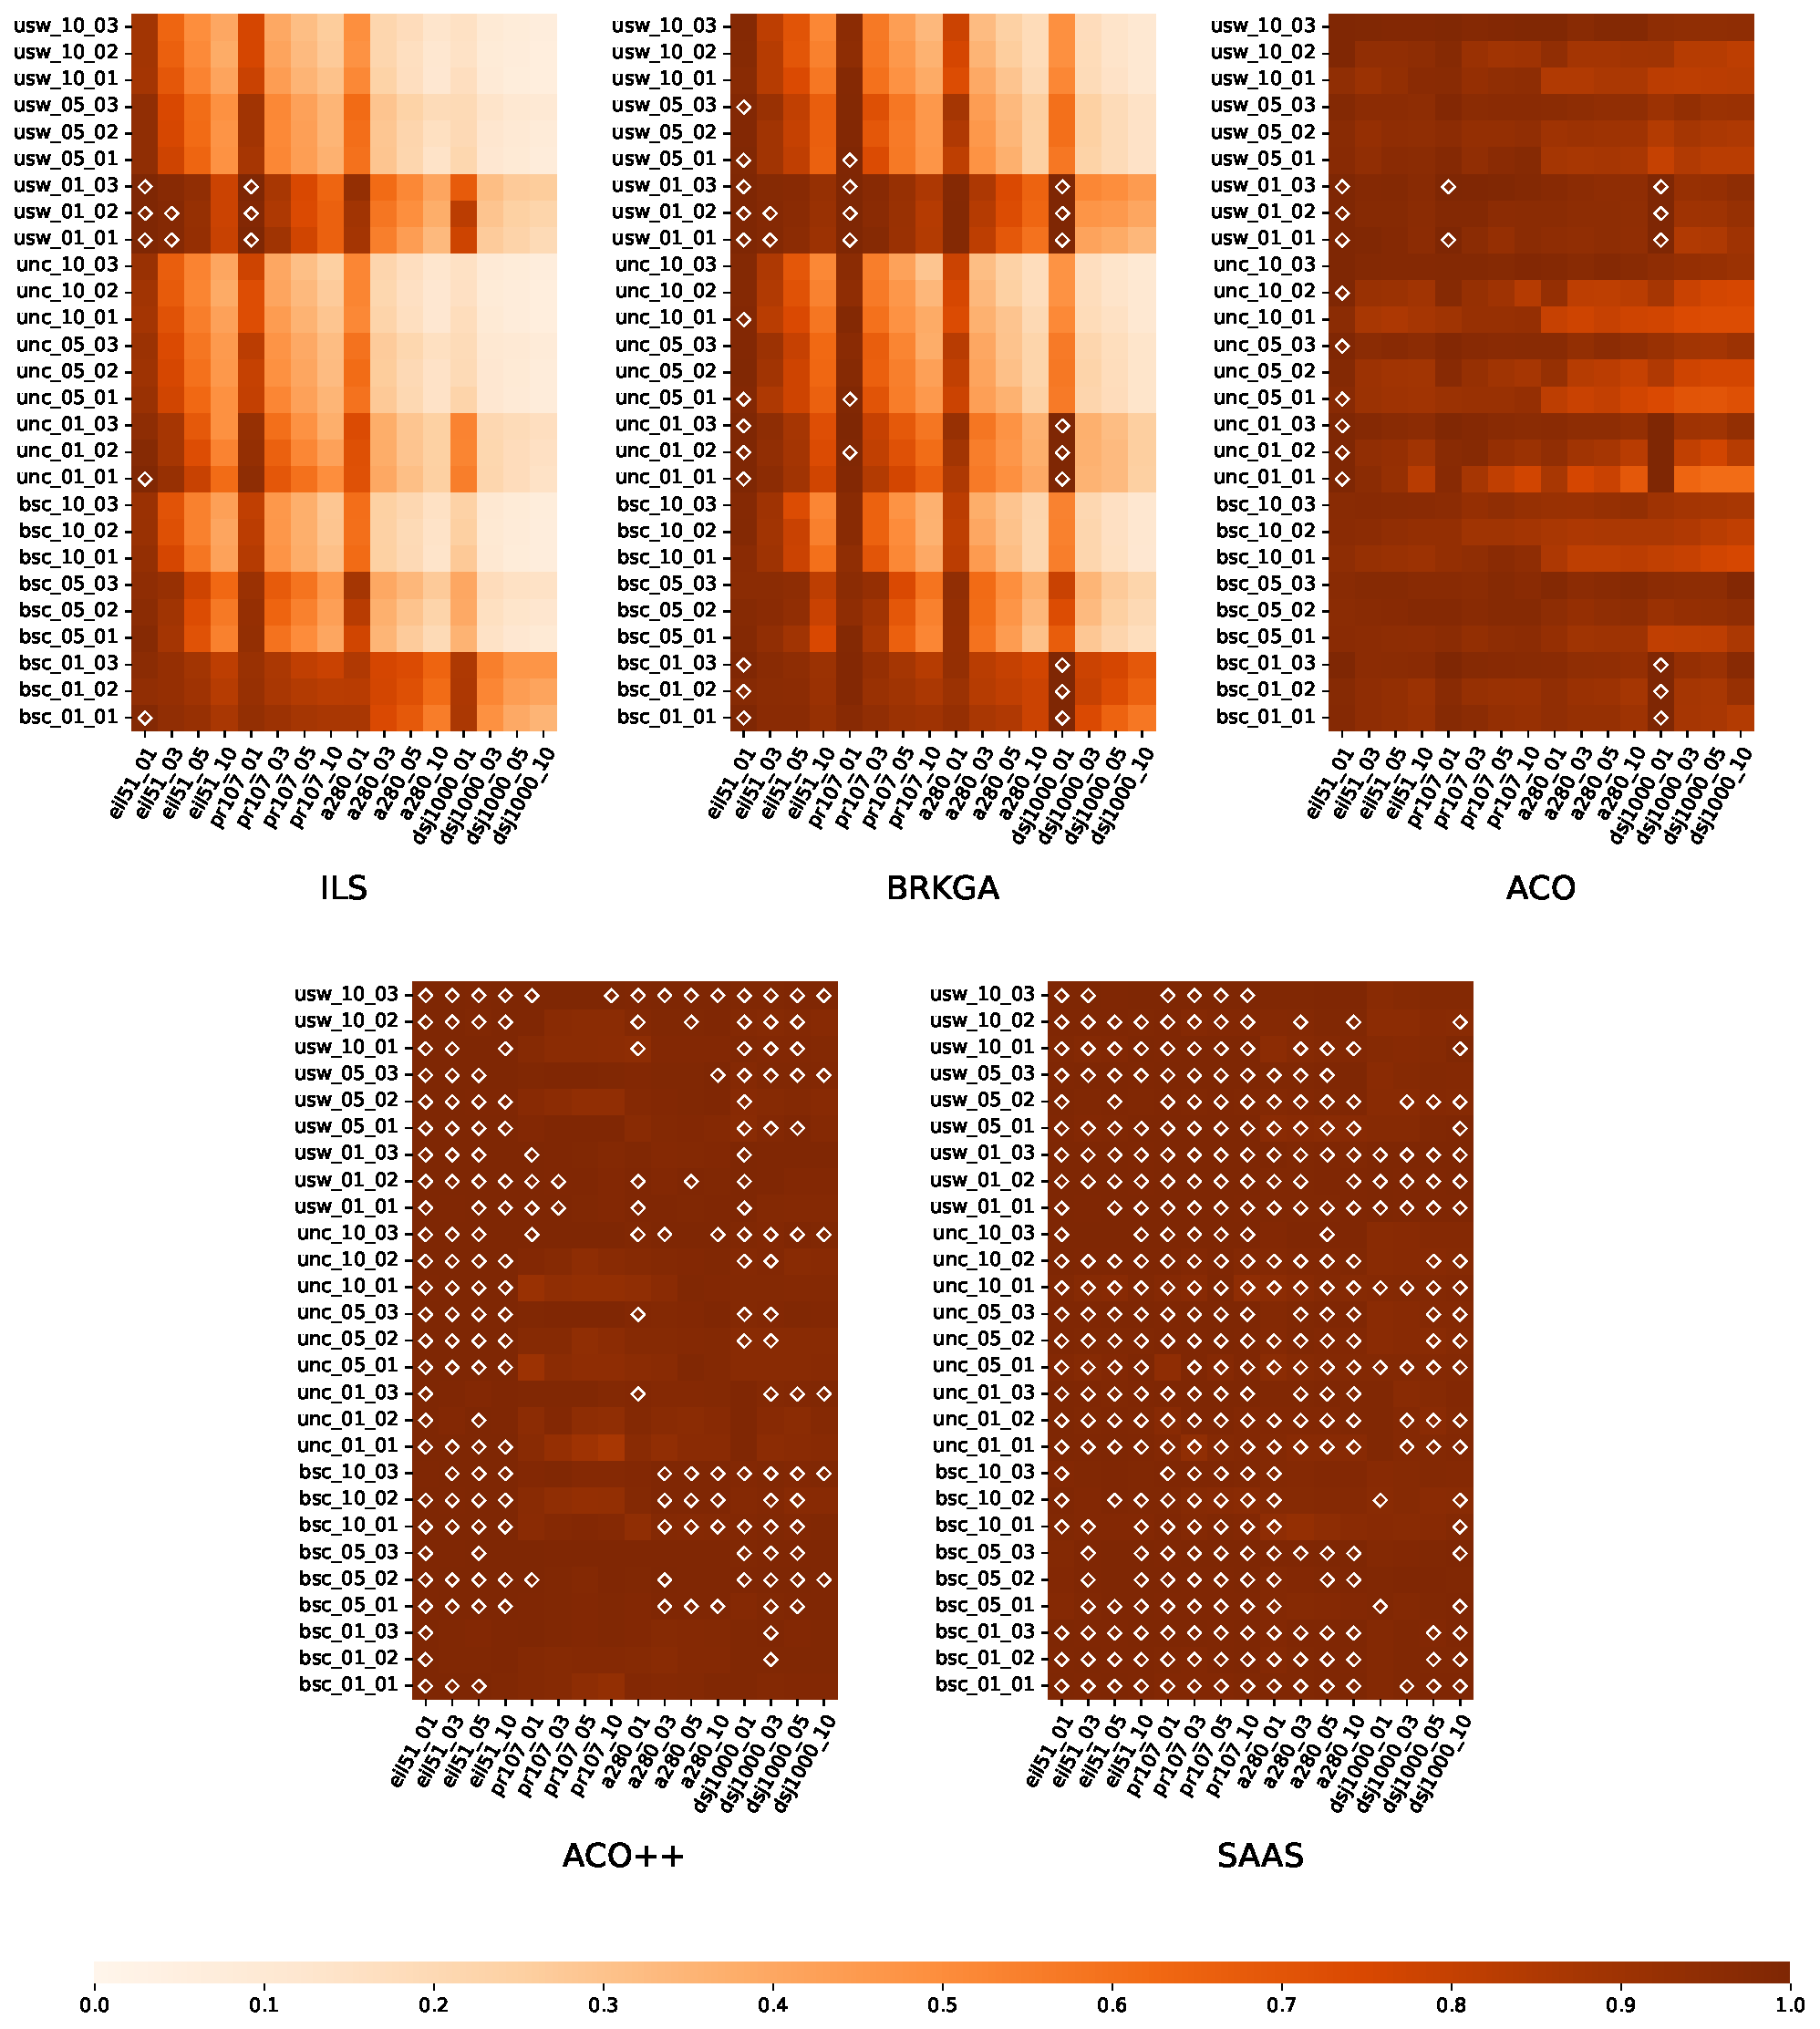
\includegraphics[width=\textwidth]{Figures/profit_ratio.pdf}
    \caption[Kết quả thực nghiệm so sánh lời giải của các thuật toán.]{Biểu đồ nhiệt của mỗi thuật toán thể hiện tỉ lệ kết quả lời giải trên từng trường hợp của thuật toán đó, với lời giải tốt nhất được tìm thấy cho trường hợp đó trong tất cả thực nghiệm. Mỗi ô trên mỗi biểu đồ nhiệt thể hiện một trường hợp. Độ đậm nhạt ở mỗi ô thể hiện tỉ lệ lời giải, màu sắc càng đậm thể hiện lời giải có kết quả gần bằng với lời giải tốt nhất được tìm thất. Ký hiệu hình thoi ở một số ô thể hiện thuật toán đó tìm ra lời giải tốt nhất được tìm thấy cho trường hợp tại vị trí đó.}
    \label{fig:profit_ratio}
\end{figure}
\subsection{Kết quả thực nghiệm so sánh hiệu suất giữa các thuật toán}
\label{sec:winpercent}
Để so sánh các cặp thuật toán với nhau về mặt số lượng lời giải tốt, chúng tôi đã xây dựng bảng \ref{tab:winpercent}, bảng thống kê phần trăm các lời giải của mỗi thuật toán tìm ra lời giải có chất lượng tốt hơn hoặc ngang bằng so với thuật toán khác. Ở mỗi cặp thuật toán, chúng tôi tính giá trị phần trăm số lượng dựa trên lời giải tốt nhất ở hai thuật toán của 30 lần chạy độc lập ở mỗi trường hợp. 

\begin{table}[ht!]
  \begin{center}      
        \begin{tabular}{lrrrrr}
        \toprule
        i $\downarrow$ \ \ \ \ j $\rightarrow$  & ILS & BRKGA & ACO & ACO++ & SAAS \\
        \midrule
        ILS & - & 2.55\% & 4.40\% & 2.55\% & 2.31\% \\
        BRKGA & 100.00\% & - & 16.20\% & 8.80\% & 7.18\% \\
        ACO & 97.22\% & 87.27\% & - & 5.79\% & 4.86\% \\
        ACO++ & 99.54\% & 95.83\% & 97.69\% & - & 41.90\% \\
        SAAS & 99.77\% & 97.92\% & 98.61\% & 78.24\% & - \\
        \bottomrule
        \end{tabular}
      \caption[Kết quả thực nghiệm so sánh hiệu suất giữa các thuật toán.]{
      \label{tab:winpercent}Bảng thống kê phần trăm chất lượng các lời giải của thuật toán i tốt hơn hoặc ngang bằng so với lời giải của thuật toán j.}
  \end{center}
\end{table}

Kết quả được thể hiện trong bảng này chứng thực cho những gì thể hiện trên hình \ref{fig:profit_ratio}. BRKGA hoàn toàn áp đảo ILS với tỉ lệ là 100\% và các thuật toán dựa trên thuật toán đàn kiến thể hiện hiệu suất tốt hơn với hai thuật ILS và BRKGA. Thuật toán của chúng tôi SAAS và ACO++ đều thiện hiện hiệu suất vượt trội so với các thuật toán khác với hơn 95\% số lượng các trường hợp trên benchmark. SAAS có số lượng lời giải tốt hơn 78.24\% ACO++. 
\subsection {So sánh thống kê Wilcoxon signed-rank}
Với hiệu suất tương đối và dẫn đầu của cả hai thuật toán SAAS và ACO++, chúng tôi tiến hành thử nghiệm Wilcoxon signed-rank để xác minh sự khác biệt giữa chúng. Sử dụng mức ý nghĩa là 5\%, kết quả cho thấy rằng hiệu suất của SAAS thấp hơn thống kê so với ACO++ ở 170 trường hợp. Trong 86 trường hợp, không có sự chênh lệch đáng kể nào được quan sát giữa hiệu suất của hai thuật toán. Ngược lại, trong 176 trường hợp, SAAS thể hiện hiệu suất ưu việt so với ACO++.

Lưu ý quan trọng rằng trong khi thuật toán SAAS có kết quả cạnh tranh với thuật toán ACO++, nó sử dụng một bộ siêu tham số duy nhất trên tất cả 432 trường hợp trong quá trình thực nghiệm trên thang đo ThOP. Ngược lại, ACO++ sử dụng 48 bộ siêu tham số riêng biệt tương ứng với 48 nhóm trường hợp trong thang đo ThOP.

\subsection{Kết quả thực nghiệm so sánh độ chênh lệch của lời giải của các thuật toán}
\label{sec:errorRate}
Hình \ref{fig:errorRate} mô tả độ chênh lệch trung bình cho các lời giải tốt nhất, tệ nhất và trung bình của các thuật toán trên tất cả các trường hợp trong thang đo ThOP. Cách chúng tôi tính các độ chênh lệch cho mỗi thuật được mô tả ở công thức \ref{eq:errorrate}. Với "ThOP benchmark" là tập các trường hợp có trong thang đo ThOP và $P_n^i$ là giá trị tổng lợi nhuận của lời giải của lần chạy độc lập thứ $n$ của trường hợp $i$.

\begin{equation}\label{eq:errorrate}
\begin{split}
    \text{Best Error} & = \frac{1}{|\text{ThOP benchmark}|}\sum_{i\in \text{ThOP benchmark}}\max(P_1^i, P_2^i, \ldots, P_{30}^i) \\
    \text{Worst Error} & = \frac{1}{|\text{ThOP benchmark}|}\sum_{i\in \text{ThOP benchmark}}\min(P_1^i, P_2^i, \ldots, P_{30}^i) \\
    \text{Average Error} & = \frac{1}{|\text{ThOP benchmark}|}\sum_{i\in \text{ThOP benchmark}}\text{mean}(P_1^i, P_2^i, \ldots, P_{30}^i) \\
\end{split}
\end{equation}

Thuật toán SAAS thể hiện hiệu suất đáng kể, với tỷ lệ chênh lệch thấp nhất là 0.14\% và 1.25\% ở các mục độ chênh lệch tốt nhất và độ chênh lệch trung bình. Mặc dù vậy độ chênh lệch trong trường hợp tồi nhất của thuật toán của chúng tôi cao hơn ACO++ khoảng 0.5\%. Mặc dù không sử dụng các bộ tham số cụ thể cho mỗi nhóm trường hợp như ACO++ đã làm, thuật toán của chúng tôi, SAAS, liên tục mang lại hiệu suất ổn định với tỷ lệ chênh lệch thấp trên tất cả ba mục.

\begin{figure}
  \centering
  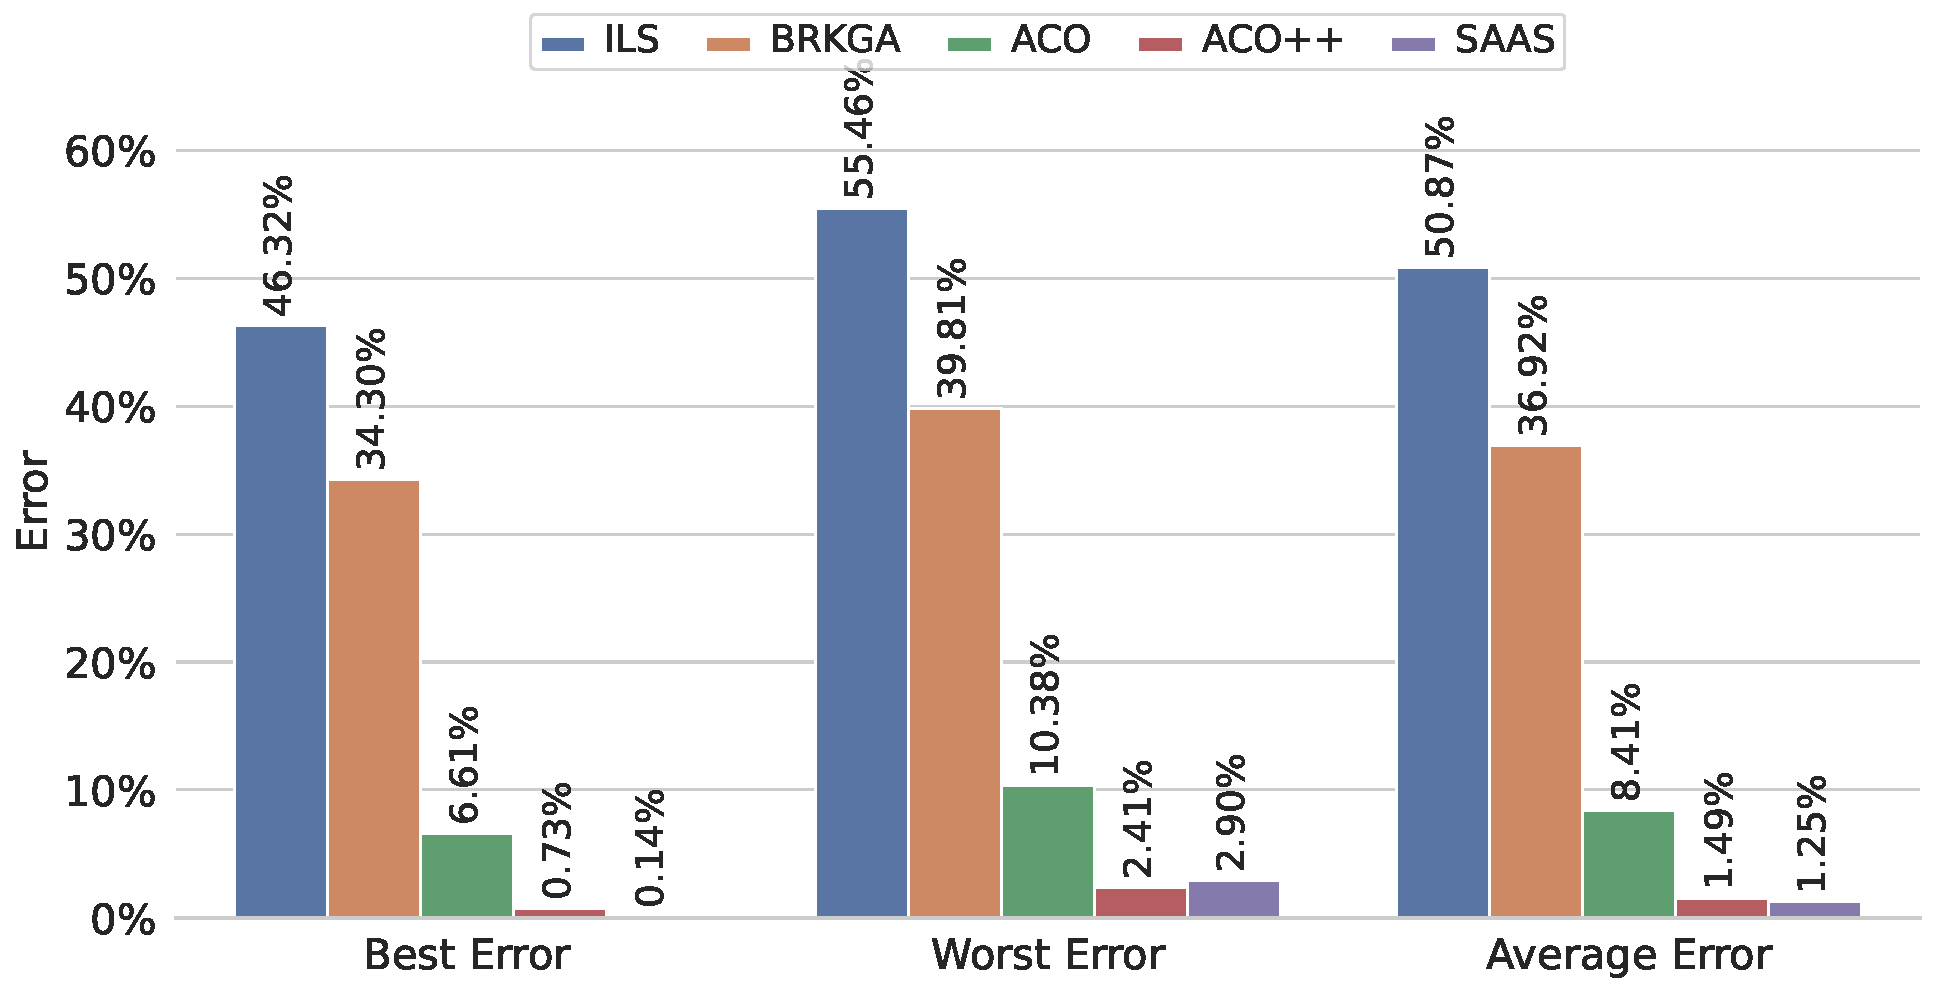
\includegraphics[width=\linewidth]{Figures/error_rate.pdf}
  \caption[Kết quả thực nghiệm so sánh độ chênh lệch của lời giải của các thuật toán.]{Biểu đồ cột thể hiện độ chênh lệch của lời giải của mỗi thuật toán so với lời giải tốt nhất tìm được. Biểu đồ thể hiện 3 cách tính độ chênh lệch: độ chênh lệch tốt nhất, độ chênh lệch tệ nhất, và độ chênh lệch trung bình.}
  \label{fig:errorRate}
\end{figure}
% \subsection{Thông tin cấu trúc của lời giải tốt nhất được tìm thấy}
% \label{sec:soltruc}
% \begin{table}
%     \begin{center}   
%         \begin{tabular}{llrrrrrrrr}
%             \toprule
%             % \multirow{2}{3em}{\texttt{XXX}} & \multirow{2}{2em}{\texttt{YY}} & \multicolumn{3}{c}{ACO++} &&  \multicolumn{3}{c}{SAAS}\\
%             \multicolumn{2}{c}{trường hợp group}& \multicolumn{3}{c}{ACO++} &&  \multicolumn{3}{c}{SAAS}\\
%             \cline{3-5}\cline{7-9}
%             \texttt{XXX} & \texttt{YY} &\multicolumn{1}{c}{$\mathcal{D}$} & \%T & \%W &&\multicolumn{1}{c}{$\mathcal{D}$} & \%T & \%W \\
%             \midrule
%             \multirow{4}{3em}{eil51}    & 01 &              10.469 &           98.994 &  \textbf{79.551} &   &     \textbf{10.447} &  \textbf{99.123} &           79.533 \\
%                                         & 03 &               8.646 &           99.592 &  \textbf{85.066} &   &      \textbf{8.636} &  \textbf{99.668} &           84.939 \\
%                                         & 05 &      \textbf{8.517} &  \textbf{99.759} &           85.412 &   &                8.53 &           99.731 &  \textbf{85.514} \\
%                                         & 10 &      \textbf{8.204} &           99.865 &  \textbf{86.544} &   &               8.243 &  \textbf{99.913} &            86.52 \\
%             \midrule
%             \multirow{4}{3em}{pr107}    & 01 &             682.053 &           99.686 &  \textbf{81.697} &   &    \textbf{663.738} &   \textbf{99.77} &  \textbf{81.697} \\
%                                         & 03 &             477.944 &  \textbf{99.931} &           83.823 &   &    \textbf{476.552} &           99.894 &  \textbf{84.443} \\
%                                         & 05 &             447.241 &           99.939 &           84.173 &   &    \textbf{437.632} &  \textbf{99.943} &  \textbf{85.575} \\
%                                         & 10 &             417.133 &           99.881 &           84.728 &   &    \textbf{414.535} &  \textbf{99.949} &  \textbf{85.576} \\
%             \midrule
%             \multirow{4}{3em}{a280}     & 01 &      \textbf{14.11} &           99.815 &  \textbf{84.743} &   &              14.155 &  \textbf{99.838} &           84.651 \\
%                                         & 03 &     \textbf{10.405} &           99.763 &  \textbf{85.825} &   &              10.462 &  \textbf{99.937} &           85.735 \\
%                                         & 05 &      \textbf{9.651} &           99.917 &            86.33 &   &               9.736 &  \textbf{99.935} &  \textbf{86.493} \\
%                                         & 10 &      \textbf{9.216} &           99.961 &           86.126 &   &               9.419 &  \textbf{99.964} &    \textbf{86.2} \\
%             \midrule
%             \multirow{4}{3em}{dsj1000}  & 01 &  \textbf{37309.633} &           72.359 &  \textbf{86.171} &   &           41557.939 &  \textbf{74.142} &           85.822 \\
%                                         & 03 &  \textbf{18960.953} &           99.937 &  \textbf{89.691} &   &           19286.319 &  \textbf{99.964} &           89.598 \\
%                                         & 05 &           18034.123 &  \textbf{99.959} &           90.059 &   &  \textbf{17868.094} &           99.795 &  \textbf{90.364} \\
%                                         & 10 &  \textbf{17694.494} &  \textbf{99.692} &  \textbf{90.497} &   &           17737.117 &           99.664 &            90.44 \\
%             \midrule
%             \multicolumn{2}{c}{Total}  & 9 & 4 & 9 && 7 & 12 & 8  \\
%             \bottomrule
%         \end{tabular}
%         \caption[Thông tin cấu trúc của lời giải tốt nhất được tìm thấy của ACO++ và SAAS]{
%         \label{tab:soltruc}Thông tin cấu trúc của lời giải tốt nhất được tìm thấy. Giá trị in đậm thể hiện yếu tố đó của thuật toán hiệu quả hơn so với thuật toán còn lại.}
%     \end{center}
% \end{table} 
\chapter{KẾT LUẬN VÀ HƯỚNG PHÁT TRIỂN} \label{chapter:Conclusion}

Chúng tôi đã cải tiến thuật toán ACO++ bằng cách tích hợp hai cơ chế kiểm soát tham số, kỹ thuật Bay hơi lười biếng và kỹ thuật Phân cụm thứ bậc để tăng cường tính linh hoạt và hiệu suất. Hầu hết các tham số của chúng tôi được điều chỉnh tự động, một số trở nên tự thích ứng nhờ vào ES và một số khác trở nên thích ứng thông qua cơ chế thích ứng lấy cảm hứng từ AACO-NC. Kiến di chuyển trên các cạnh của cây cụm thứ bậc thay vì di chuyển từ thành phố này sang thành phố khác. Phân cụm thứ bậc đã giúp làm giảm chi phí tìm kiếm tuyến đường. Bay hơi lười biếng giúp giảm thiểu độ phức tạp thời gian của giai đoạn bay hơi bằng cách theo dõi trạng thái mong muốn và lịch sử, và chỉ bay hơi pheromone trên các cạnh được sử dụng. Trong khi ACO++ yêu cầu điều chỉnh riêng cấu hình siêu tham số cho mỗi nhóm trường hợp, SAAS mang lại kết quả xuất sắc với chỉ một cấu hình chạy trên tất cả 432 trường hợp đánh giá.

Trong công trình này, chúng tôi chỉ mới tập trung cải tiến ở giai đoạn tìm đường và chất lượng của tham số. Ở bài toán Điều Hướng Thu Thập và các thuật toán trước đó, tồn tại hai giai đoạn quan trọng khác mà chúng tôi chưa chạm đến. Đó là xây dựng chiến lược thu thập và tìm kiếm cục bộ. Các thuật toán cho bài toán Người Thu Thập Du Lịch (TTP) sở hữu các phép tìm kiếm cục bộ rất truyền cảm hứng \cite{Namazi2023SolvingTT}. Ta có thể điều chỉnh chúng để áp dụng được cho ThOP. Chiến lược thu thập của SAAS, được kế thừa từ ACO++, có độ phức tạp cao nhất trong tất cả giai đoạn, chứa nhiều khả năng có thể cải tiến.

Bộ trường hợp đánh giá của ThOP rất đa dạng và bao phủ rộng các khả năng. Tuy vậy, nó vẫn tồn tại vài thiếu sót không giống với thực tế. Ví dụ như mỗi thành phố đều có số lượng vật phẩm như nhau và bản đồ mang tính đối xứng. Bản đồ đối xứng nghĩa là quãng được từ A đến B và từ B đến A là như nhau. Điều này có thể dẫn đến đánh giá sai tiềm năng của thuật toán trong bối cảnh thực tế. Các nghiên cứu tương lai có thể hướng đến cải thiện yếu điểm này.

Các kĩ thuật chúng tôi đề xuất có khả năng tích hợp vào các phương pháp tân tiến trên nhiều bài toán khác, từ đó giúp cải thiện chất lượng lời giải. Ta cũng có thể tích hợp các yếu tố cửa sổ thời gian (time window), nhiều điểm kho chứa (multiple depot) hoặc đa mục tiêu vào bài toán Điều Hướng Thu Thập để thúc đẩy bài toán nghiên cứu gần hơn với vấn đề thực tế. 


%----------------------------------------------------------------------------------------
%	THESIS CONTENT - APPENDICES
%----------------------------------------------------------------------------------------

% \appendix % Cue to tell LaTeX that the following "chapters" are Appendices

% Include the appendices of the thesis as separate files from the Appendices folder
% Uncomment the lines as you write the Appendices

%% Appendix A

\chapter{Frequently Asked Questions} % Main appendix title

\label{AppendixA} % For referencing this appendix elsewhere, use \ref{AppendixA}

\section{How do I change the colors of links?}

The color of links can be changed to your liking using:

{\small\verb!\hypersetup{urlcolor=red}!}, or

{\small\verb!\hypersetup{citecolor=green}!}, or

{\small\verb!\hypersetup{allcolor=blue}!}.

\noindent If you want to completely hide the links, you can use:

{\small\verb!\hypersetup{allcolors=.}!}, or even better: 

{\small\verb!\hypersetup{hidelinks}!}.

\noindent If you want to have obvious links in the PDF but not the printed text, use:

{\small\verb!\hypersetup{colorlinks=false}!}.

%\include{Appendices/AppendixB}
%\include{Appendices/AppendixC}

%----------------------------------------------------------------------------------------
%	BIBLIOGRAPHY
\addchaptertocentry{\bibname}
\printbibliography
%----------------------------------------------------------------------------------------
\end{document}  
